\RequirePackage[l2tabu,orthodox]{nag}
\documentclass[bachelors,a4paper,gu]{chalmers-thesis}
\usepackage[firstinits=true,style=alphabetic,backend=biber]{biblatex}
\usepackage[swedish,english]{babel}
\usepackage[utf8]{inputenc}
\usepackage{amsfonts,amsmath,amsthm}
\usepackage{caption}
\usepackage{color}
\usepackage{csquotes}
\usepackage{float}
\usepackage{hyperref}
\usepackage{listings}
\usepackage{mathtools}
\usepackage{microtype}
\usepackage{subfig}
\usepackage{subfiles}
\usepackage{tikz}
\usepackage{url}
\usepackage{verbatim}
\usepackage{xspace}

\newcommand{\coq}{{\sc Coq}}
\newcommand{\ssr}{{\sc SSReflect}}
\newcommand{\C}[1]{\mbox{\lstinline`#1`}}
\let\L=\lstinline

\definecolor{dkblue}{rgb}{0,0.1,0.5}
\definecolor{lightblue}{rgb}{0,0.5,0.5}
\definecolor{dkgreen}{rgb}{0,0.4,0}
\definecolor{dk2green}{rgb}{0.4,0,0}
\definecolor{dkviolet}{rgb}{0.6,0,0.8}
\definecolor{shadethmcolor}{rgb}{0.9, 0.9,1}

\def\lstlanguagefiles{defManSSR.tex}
\lstset{language=SSR}

\lstset{moredelim=[is][\color{red}\bfseries\ttfamily\underbar]{|*}{*|}}
%Highlights metalevel expressions in italic rm font
\lstset{moredelim=*[is][\itshape\rmfamily]{/*}{*/}}

%\theoremstyle{plain}
%\theorembodyfont{\upshape}
%\newshadetheorem{exercise}{Exercise}[subsection]

\newcommand{\Ordo}{\mathcal{O}}

\newtheorem{theorem}{Sats}[section]
\newtheorem{definition}[theorem]{Definition}
\newtheorem{lemma}[theorem]{Lemma}
\newtheorem{proposition}[theorem]{Proposition}
\newtheorem{corollary}[theorem]{Korollarium}

\DeclareMathOperator*{\grad}{grad}
\DeclareMathOperator*{\modu}{mod}

\DeclarePairedDelimiter{\floor}{\lfloor}{\rfloor}
\DeclarePairedDelimiter{\ceil}{\lceil}{\rceil}


\title{Formalisering av Algoritmer och Matematiska Bevis}
\subtitle{And stuff...}
\author{Jesper Andersson\and Daniel Oom\and Niclas Ståhl\and Åsa Lideström\and Anders Sjöberg}
\thesisin{Datateknik och Matematik}
\department{Datateknik och Matematik}
\reportno{2013:11}
\copyrightyear{2013}

\coverfigure{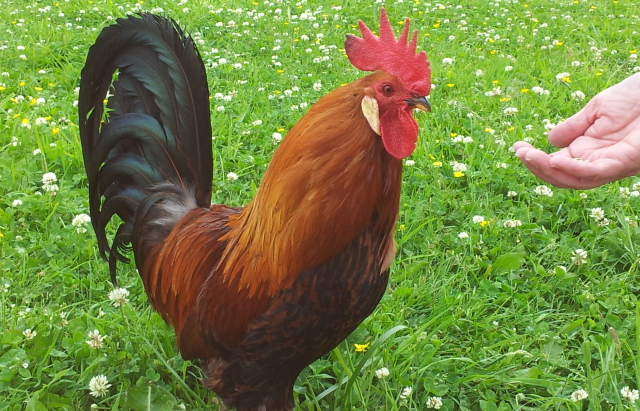
\includegraphics[width=\textwidth,height=\paperheight,keepaspectratio]{figures/Tupp}}
\covercaption{Some explanation}

\firstabstract{Utvecklingen av datorstödd formalisering av matematik har gått framåt det
senaste decenniet med formaliseringen av mycket långa och komplicerade bevis
såsom beviset för fyrfärgssatsen och Feit-Thompsons sats. I den här rapporten
presenterar vi ett formellt bevis för algoritmen Toom-Cook med hjälp av
bevisassistenten \coq{} tillsammans med tillägget \ssr{}. Toom-Cook är en algoritm
för att multiplicera polynom och kan även användas för att multiplicera heltal.

% anledning varför vi har gjort det här + resultat + diskussion
}
\secondabstract{english}{Computer-aided formalization of mathematics has taken a leap forward in the
last decade with the formalization of very large and complex proofs such as the
four colour theorem and the Feit-Thompson theorem. In this report we present a
formal proof of the \toom algorithm using the Coq proof assistant together with
the \ssr extension. The \toom algorithm is used to multiply polynomials and can
also be used for integer multiplication.
}
\keywords{Formalisering, Polynommultiplikation, Toom-Cook, \coq, \ssr}

\DeclareFieldFormat[article]{title}{#1}
\DeclareFieldFormat[article]{volume}{\mkbibbold{#1}}
\renewbibmacro{in:}{}
\DeclareFieldFormat[article]{pages}{#1}
\renewbibmacro*{journal+issuetitle}{
  \usebibmacro{shortjournal}
  \setunit*{\addspace}
  \iffieldundef{series}{}{\newunit\printfield{series}\setunit{\addspace}}
  \usebibmacro{volume+number+eid}
  \setunit{\addspace}
  \usebibmacro{issue+date}
  \setunit{\addcolon\space}
  \usebibmacro{issue}
  \newunit}

\addbibresource{report.bib}

%\pagestyle{fancy}
%\lhead{Formalisering av Algoritmer och Matematiska Bevis}
%\rhead{Grupp 11}

\begin{document}
\selectlanguage{swedish}
\maketitle

\chapter{Inledning}
Under senare år har några mycket långa och komplexa matematiska bevis
presenterats. Vissa bevis har också byggt på en mycket omfattande analys av
tusentals fall utförd av datorprogram. Det är mycket tidsödande och svårt, om
ens praktiskt möjligt att för hand kontrollera varje steg ett sådant bevis. Få
matematiker har tid, lust och den speciella kompetensen inom just det specifika
matematiska området som gör att de kan eller vill att ägna år åt att
kontrollera att ett sådant bevis är korrekt. Dessutom finns risken för att ett
fel i ett bevis ändå inte upptäcks vid kontroll om beviset är hundratals- eller
tusentals sidor långt\cite{harrison2008formal}.

Bevisassistenter, datorsystem för att formalisera och verifiera varje logiskt
steg i bevis, kan användas för att kontrollera bevis och därmed minska risken
för att de innehåller fel och öka tilltron till att de är korrekta.

Fyrfärgssatsen\cite{gonthier2008formal} och Feit-Thompsons
sats\cite{aschbacher2004status} är två exempel på satser vars bevis har
formaliserats och kontrollerats i bevisassistenter. Fyrfärgssatsen säger att
varje karta kan färgläggas med fyra färger så att inga regioner med gemensam
gräns får samma färg. Det ursprungliga beviset var över hundra sidor långt och
byggde också datorprogrammerad fallanalys av miljontals fall. Detta gjorde
beviset svårt att kontrollera och kontroversiellt. Beviset formaliserades och
verifierades i bevisassistenten \coq 1995.
%Lite mer om fyrfärgssatsen här?
%Lite mer om Odd order theorem här?

De verktyg som används vid formalisering och datorverifiering kan även användas
för att verifiera programkod. Formella metoder är således intressant för både
för programmerare och matematiker.
% Niclas: Den här meningen säger väldigt lite. Varför??
Dagens stora och komplexa programvaror skulle kunna utnyttja formella metoder.
%)
Det kan också vara användbart i kritiska system, till exempel medicinsk
utrustning, där det inte får bli fel eller i system som inte kan uppdateras i
efterhand som hårdvarunära mjukvara på ROM-minnen.

De mest använda metoderna idag för att kontrollera kod bygger på att testa om
koden ger korrekt resultat för olika indata. På detta sätt har man en chans att
upptäcka om koden innehåller fel, men det visar inte att koden saknar fel
eftersom det i många fall är omöjligt att testa alla kombinationer av indata.
% Niclas: + Svårt/Krävande att hitta kända resultat?
Formella metoder skulle i dessa fall kunna användas till att garantera
korrekthet hos koden.

Ett exempel på projekt för att verifiera kod är CompCert. Det utforskar
möjligheten att utveckla formellt bevisade kompilatorer. Anledningen att man
vill ha en formellt bevisad kompilator är att vid vissa optimeringar så kan
kompilatorn skapa buggar och beräkningsfel. Huvudresultatet av detta är en
fungerande C-kompilator som är bevisad i \coq och som stödjer hela ANSI C (som
är den första standardiserade versionen av C) med få
undantag\autocite{compcert}.

Matematisk programvara som MATLAB spelar en stor roll för beräkningar inom
forskning och industri och det finns därmed ett stort intresse av att de är
% Niclas: känns som det kan finnas bättre ord än buggfria
pålitliga. De är dock inte buggfria. Ett sätt att göra dem mer pålitliga skulle
vara att formalisera de ingående algoritmerna och visa att de är korrekt
implementerade\cite{denes2012refinement}.

Det här projektet går ut på att gruppdeltagarna ska lära sig formalisering med
bevisassistenten \coq och sedan formalisera och bevisa en matematisk algoritm,
\toom, i \coq.

\coq är en av flera avancerade bevisassistenter som det bedrivs aktiv forskning
om. Några andra är Agda, som utvecklats på Chalmers, Z3, som har utvecklats av
Microsoft och kan användas tillsammans med flera stora ickefunktionella språk
som Python, C och .NET och HOL-light, som används av Intel för att bevisa att
vissa hårdvarukomponenter fungerar korrekt och i det pågående projektet att
formalisera Keplers förmodan \cite{hales2008formal}.

\toom är en algoritm för att multiplicera heltal eller polynom. Den är
intressant eftersom den har en bättre asymptotisk tidskomplexitet än
polynommultiplikation utförd direkt enligt definitionen \footnote{För
definition av polynommultiplikation, se
appedix~\ref{appendix:matematikteori}.}, där man multiplicerar varje term i det
ena polynomet med varje term i det andra polynomet vilket har den asymptotiska
tidskomplexiteten $O\left(n^2\right)$\footnote{Funktionen $T(n)$ är $O(f(n))$
om det existerar konstanter $c > 0$ och $n_0 \geq 0$ så att $T(n) \leq c \cdot
f(n)$ för alla $n \geq n_0$.}, där n är graden på det största av de två
polynomen som skall multipliceras.


\newpage
\chapter{Metod/Genomförande}
Följande avsnitt beskriver tillvägagångssättet för formalisering av algoritmen.

\section{Litteraturstudie och färdighetsträning}
Som första steg i arbetet utfördes en studie med mål att få tillräckligt med
kunskaper för att programmera och bevisa med hjälp av \coq{} och \ssr{}. Som
material användes bland annat \emph{Software Foundations} av Benjamin C. Pierce
som är kursmaterial till en grundkurs i \coq{}, \emph{Coq in a Hurry} av Yves
Bertot som är en kort introduktionsartikel till \coq{} och \emph{SSReflect
tutorial} av Georges Gonthier som är en introduktion till \ssr{}. Som övning
gjordes även ett bevis av Karatsuba-algoritmen i \coq{}.

\section{Definition och bevis för hand}
Först gjordes en informell men detaljerad definition av en generell och
abstrakt version av Toom-Cook. Med abstrakt menas utan hänsyn till om det går
att implementera. Ett detaljerat bevis gjordes också på papper för senare
användning i implementationen.

\section{Implementation i \haskell{}}
I samband med framtagningen av det informella beviset utvecklades en praktisk
implementation av Toom-Cook för heltal i \haskell{}. Den byggdes först för
Toom-Cook-3 men generaliserades sedan till \toomp{n}. Testning gjordes med
QuickCheck genom att jämföra implementationen av Toom-Cook med
heltalsmultiplikationen som finns definierad i \haskell{}. Resultatet av denna
fasen finns i appendix~\ref{app:haskell}.

Anledningen till att en implementation gjordes i \haskell{} var för att vi i det
stadiet inte hade tillräckligt med kunskap om \coq{} för att implementera en ny
algoritm i språket. Eftersom erfarenhet av \haskell{} redan fanns kunde algoritmen
snabbt implementeras och testas, detta gav också en bättre förståelse för hur
Toom-Cook fungerar.

\section{Implementering och bevis i \coq{}}
När informella beviset och den praktiska implementation var färdiga, utfördes
implementeringen av Toom-Cook och dess bevis i \coq{} med hjälp av \ssr{}.
Först skapades en definition av algoritmen i \coq{} väldigt lik den i
\haskell{} fast med polynom istället för heltal. Denna definition omarbetades
senare under bevisningen för att det skulle vara lättare att arbeta med
beviset. Uppdelningen av lemmana gjorde det möjligt. Resultatet av detta
beskrivs i avsnitt~\ref{sec:formellimplementation} och
avsnitt~\ref{sec:formellbevis}.

\section{Avgränsningar}
Från början var tanken att en optimerad version av Toom-Cook skulle
implementeras och jämföras med lång multiplikation men i brist på tid gjordes
aldrig detta. Vår implementation kan således inte användas, utan vi \emph{vet}
bara att den är korrekt.


\newpage
\chapter{Bevisassistenter och formalisering av matematik}
\coq{} är en \emph{bevisassistent} som används för att formalisera och bevisa
matematik och kod.
% Denna meningen känns lite märklig jag antar "och formalisera bevis för att
% den är korrekt är kopplad till kod, men det är inte så tydligt //J
I det här avsnittet ges en introduktion till vad ett matematiskt bevis är och
vad som menas med formalisering av matematik. Sedan beskrivs vad en
bevisassistent är och kan göra.

\section{Matematiska bevis och datorverifiering}
Vanlig matematisk text är en blandning mellan formler och naturligt språk. Ett
matematiskt bevis i en kursbok eller vetenskaplig artikel kan sägas vara en
skiss av ett fullständigt bevis, ett argument, som ska övertyga läsaren om att
satsen är korrekt och beviset är giltigt. Varje litet logiskt bevissteg behöver
inte tas med, särskilt inte om den avsedda läsaren är van vid typen av bevis
som det handlar om. Dessa steg kan läsaren själv fylla i.

%Exempel andragradsekvation?

Det är också vanligt att många saker får framgå av sammanhanget.
% Kan man formulera det annorlunda än "låter många saker"? //J
Till exempel kan symbolen 1 stå för olika saker, bland annat det naturliga
talet 1 som är efterföljare till 0, det rationella talet $\frac{1}{1}$ eller
det multiplikativa enhetselementet i en ring\footnote{För en definition av
ringar, se appendix~\ref{sec:algebra}}. Oftast kan en mänsklig läsare ur
sammanhanget förstå vilken betydelse av 1 som avses i ett visst fall.
%fast coq kan ju också göra typinferens

För att ett datorsystem ska kunna kontrollera bevis krävs att det finns en
exakt definition av vad det innebär att ett bevis är giltigt. En definition är
att
\begin{quote}
``... the correctness of a mathematical text is verified by comparing it, more or
less explicitly, with the rules of a formalized language'' -- \cite{bourbaki1968sets}.
\end{quote}
% TODO: Översätta citatet?

Givet den definitionen måste ett bevis \emph{formaliseras} för att ett
datorsystem mekaniskt ska kunna kontrollera det. Det innebär att sådant som en
mänsklig läsare förstår ur sammanhanget måste göras explicit och bevissteg som
är så små att de ses som självklara för en människa måste också skrivas ut.

Datorsystemet kan sedan kontrollera om varje steg i beviset följer från
föregående steg eller från axiom genom en bestämd mängd fastslagna
\emph{härledningsregler}. Dessa är enkla logiska regler om hur man får gå från
givna premisser till slutsatser. Till exempel säger härledningsregeln
\emph{modus ponens} att man ur förutsättningarna $A$ och $A \to B$ får dra
slutsatsen att $B$ gäller. Systemet kontrollerar också om de uttryck man
skriver in är tillåtna, det vill säga om man använt rätt syntax.
$\forall 3^{\frac{+}{\in}} \leftrightarrow =$ är till exempel inget välformat
uttryck. Det har ingen matematisk betydelse även om de ingående symbolerna är
matematiska och logiska symboler. Ett annat exempel på felaktig syntax eller
felformade uttryck är om man försöker definiera en funktion
\begin{lstlisting}
exempel_funktion (n : nat) : bool := n + 2.
\end{lstlisting}
eller med matematisk notation
\begin{align*}
  exempel\_funktion :\ &\mathbb{N} \to \{sant, falskt\} \\
                       &n \mapsto n + 2
\end{align*}
som enligt specifikationen ska gå från naturliga tal (\C{nat}) till boolska
sanningsvärden (\C{bool}) men som samtidigt sägs ska anta värdet $n + 2$ för
varje naturligt tal $n$.

För att formalisera matematik i en bevisassistent måste man alltså bestämma de
exakta reglerna som bevisassistenten ska följa:
\begin{itemize}
  \item vilka härledningsregler som ska vara tillåtna,
  \item vilka axiom som skall användas,
  \item vilka symboler det är tillåtet att forma uttryck med,
  \item och vilka uttryck av dessa symboler som är godkända.
\end{itemize}
Eftersom det finns olika möjliga val för alla dessa punkter finns det olika
\emph{formella språk} eller \emph{logiska system}. Ett val av en uppsättning
härledningsregler, axiom och regler för vilka symboler och uttryck som är
tillåtna ger oss \emph{ett} möjligt logiskt system.

De flesta logiska system som används för att formalisera matematik kan dock
uttrycka och härleda ungefär samma matematik och logik, möjligen på något olika
sätt, eftersom skaparna har varit intresserade av att fånga och beskriva
naturliga logiska resonemang.

En viktig skillnad är dock den mellan intuitionistisk och klassisk logik. En
utvidgning av \emph{intuitionistisk typteori}\cite{martin1984intuitionistic} är
det logiska system som finns i grunden till \coq{}\cite{bertot2004interactive}.
Det går att se den som en bevisbarhetslogik. Skillnaden mellan den och klassisk
logik kan illustreras genom följande exempel: I klassisk logik är det en logisk
sanning att $A \lor \neg A$ gäller för alla satser $A$ \footnote{Detta brukar
kallas lagen om det uteslutna tredje.}. Så om $A$ inte är sann måste $\neg A$
vara sann\cite{bennet2004forsta}.

I intuitionistisk logik däremot låter vi ``$A$ är giltig'' betyda ``det finns
ett bevis för $A$''. Om $A$ inte är giltig finns det alltså inget bevis för
$A$. Men bara för att det inte finns något bevis för $A$ betyder det inte att
det i stället nödvändigtvis finns ett bevis för $\neg A$. Detta betyder att
vissa motsägelsebevis som är giltiga i klassisk logik inte kommer vara giltiga
i intuitionistisk logik\cite{barendregt2001proofdependent}.

Om vi i klassisk logik har antagit att $\neg A$ gäller och visat att detta
leder till en motsägelse så kan vi, eftersom då $A \lor \neg A$ är en logisk
sanning måste minst en av $A$ och $\neg A$ måste gälla, därmed dra slutsatsen
att $A$ gäller.

\section{Bevisassistenter}
Ovan diskuteras vad som krävs för att ett datorsystem ska kunna kontrollera
giltigheten i matematiska bevis. De tidigaste bevissystemen för datorer kunde
endast göra detta så användaren var själv tvungen att skriva in varje enskilt
logiskt steg i det formella beviset, medan datorsystemet bara passivt
kontrollerade att dessa var giltiga.

Senare system ger användaren möjligheten att i stället skriva ett
\emph{bevisskript}, som är en rad instruktioner till systemet som talar om hur
det ska bygga upp det formella beviset, utan att användaren själv behöver mata
in varje enskilt logiskt steg.
% Vad menas med taktiker, har vi förklarat tactic tidigare? //J
% Du har rätt, jag försöker få in det.
Instruktionerna i bevisskripet kan ha formen av \emph{taktiker}, som säger till
bevisassistenten vilken form av bevisstrategi som ska användas under olika steg
i beviset. Till exempel kan användaren instruera bevisassistenten om att
beviset ska göras med taktiken induktion över någon parameter i satsen.

Användaren kan skriva bevisskriptet interaktivt. Då ger användaren
taktikinstruktionerna till systemet en i taget. Efter varje instruktion
kontrollerar systemet om taktiken gick att genomföra, och efter varje genomförd
taktik uppdaterar systemet informationen som visas för användaren om var i
beviset man nu befinner sig och vad som återstår att bevisa. Bevisassistenten
bygger på detta sätt steg för steg upp det formella beviset efter
instruktionerna från användaren och kontrollerar efter hand att de ger upphov
till ett korrekt bevis.
% Typcheckning av bevisobjektet finns också i vissa bevisassistenter, men jag vet inte
% om det är så i alla.
Bevisassistenter kan utformas så att användaren kan ange att vissa steg i
beviset ska lösas automatiskt eftersom de är så enkla att systemet själv kan
hitta de härledningsregler och axiom som krävs för att visa dem.

% Kan man få in ordet interaktiv och mer tydligt förklara vad det innebär
% att en bevisassistent är interaktiv. //J Nu har jag försökt. Å

Helt automatiserade bevismaskiner finns också. Då behöver användaren bara
formulera ett antagande, och systemet söker sedan själv efter ett bevis för
detta. De klarar dock ofta inte av att hitta komplicerade matematiska bevis
inom skiljda matematiska
områden\cite{geuvers2009proof}\cite{gonthier2009ssreflect}.
%Sista meningen är lite luddig, för jag vet egentligen inte vad som gäller.


\newpage
\chapter{\coq}
\section{\coq kod}
\label{sec:coqkod}
\begin{lstlisting}
Require Import ssreflect ssrbool eqtype ssrnat ssrfun.
Require Import seq tuple choice.
Require Import finalg finfun fingroup finset fintype.
Require Import bigop matrix ssralg.
Require Import mxpoly poly polydiv.
Require Import div zmodp.

Set Implicit Arguments.
Unset Strict Implicit.
Unset Printing Implicit Defensives.

Import GRing.Theory Pdiv.Ring Pdiv.CommonRing Pdiv.RingMonic.
Open Scope ring_scope.

Section toomCook.
Check Set.
Check Type.

Variable R : idomainType.
Implicit Types p q : {poly R}.

Variable number_splits : nat.
Definition m : nat := number_splits.
Definition number_points := (2 * m) .-1.
Variable inter_points : 'cV[{poly R}]_(number_points).

Hypothesis m_neq_0 : 0 < m.

Definition V_e : 'M[{poly R}]_(number_points, m) :=
  \matrix_(i < number_points, j < m) ((inter_points i 0))^+j.

Definition V_I : 'M[{poly R}]_(number_points) :=
 \matrix_(i < number_points, j < number_points) ((inter_points i 0))^+j.

Hypothesis unitV_I : unitmx V_I.

Definition exponent (m: nat) p q : nat :=
  (maxn (divn (size p) m) (divn (size q) m)).+1.

Definition split (n b: nat) p : {poly {poly R}} :=
  \poly_(i < n) rmodp (rdivp p 'X^(i * b)) 'X^b.

Definition evaluate (u: {poly {poly R}}) : 'cV[{poly R}]_(number_points) :=
  V_e *m (poly_rV u)^T.

Definition interpolate (u: 'cV[{poly R}]_(number_points)) : {poly {poly R}} :=
  rVpoly (invmx V_I *m u)^T.

Definition recompose (b: nat) (w: {poly {poly R}}) : {poly R} :=
  w.['X^b].

Fixpoint toom_cook_rec (n: nat) p q : {poly R} :=
  match n with
  | 0%N => p * q
  | n'.+1 => if (size p <= 2) || (size q <= 2) then p * q else
        let b := exponent m p q in
        let u := split m b p in
        let v := split m b q in
        let u_a := evaluate u in
        let v_a:= evaluate v in
        let w_a := \col_i toom_cook_rec n' (u_a i 0) (v_a i 0) in
        let w := interpolate w_a
         in recompose b w
  end.

Lemma split_size_leq_m: forall (p: {poly R}) (b: nat),
 size (split m b p) <= m.
Proof.
 by move=> p b; rewrite size_poly.
Qed.

Lemma matrix_evaluation : forall p (b: nat),
  evaluate (split m b p) = \col_j (split m b p).[(inter_points j 0)].
Proof.
move=> p b.
apply/matrixP => i j.
rewrite !mxE /=.
rewrite (@horner_coef_wide _ m).
apply: eq_bigr => k _.
by rewrite !mxE mulrC.
by apply: split_size_leq_m.
Qed.

Lemma toom_cook_interpol_lemma0 : forall (f: {poly {poly R}}),
  size f <= number_points ->
  unitmx V_I ->
  invmx V_I *m \col_i f.[inter_points i 0] = (poly_rV f)^T.
Proof.
  move=> f fsizeH unitV_I2.
  rewrite -[X in _ = X](mulKmx unitV_I2).

  have->: \col_i f.[inter_points i 0] = V_I *m (poly_rV f)^T.
    apply/matrixP => i j.
    rewrite !mxE (@horner_coef_wide _ number_points).
    apply: eq_bigr => k _.
    by rewrite !mxE mulrC.
    by apply: fsizeH.
  done.
Qed.

Lemma toom_cook_interpol : forall (f: {poly {poly R}}),
  size f <= number_points -> unitmx V_I ->
  (interpolate (\col_i (f.[(inter_points i 0)]))) = f.
Proof.
  move=> f leq unitV_I2.
  by rewrite -{2}(poly_rV_K leq) /interpolate 
   (toom_cook_interpol_lemma0 leq unitV_I2) trmxK.
Qed.

Lemma rdivpXn_drop : forall p n, rdivp p 'X^n = Poly (drop n p).
Proof.
elim/poly_ind=> [n|p c ih [|n]]; first by rewrite rdiv0p polyseq0.
  rewrite expr0 rdivp1 drop0; apply/poly_inj.
  by rewrite (@PolyK _ 1 (p * 'X + c%:P)) //; case: (p * 'X + c%:P).
rewrite {1}[p](rdivp_eq (monicXn _ n)) mulrDl -mulrA -exprSr -addrA.
rewrite rdivp_addl_mul_small ?rmodp_addl_mul_small ?monicXn //.
  rewrite -cons_poly_def ih polyseq_cons.
  by have [-> /=| //] := nilP; rewrite polyseqC; case: (c == 0).
rewrite size_polyXn size_MXaddC ltnS; case: ifP => // _.
by rewrite (leq_trans (ltn_rmodpN0 _ _)) ?monic_neq0 ?monicXn ?size_polyXn.
Qed.

Lemma drop_addn : forall n m (s : seq R) , drop (m + n) s = drop m (drop n s).
Proof.
by elim=> [m s|m ih n [] //= a l]; rewrite ?addn0 ?drop0 // addnS ih.
Qed.

Lemma last_drop c n (s : seq R) : n < size s -> last c (drop n s) = last c s.
Proof.
elim/last_ind: s => //= s a _ hs.
by rewrite drop_rcons ?last_rcons; rewrite size_rcons ltnS in hs.
Qed.

Lemma recompose_split_lemma0 p m n :
  rdivp p ('X^m * 'X^n) = rdivp (rdivp p 'X^m) 'X^n.
Proof.
rewrite -exprD !rdivpXn_drop drop_addn.
by apply/polyP=> i; rewrite ?(coef_Poly,nth_drop) addnCA.
Qed.

Lemma rdivXn_size p n : size (rdivp p 'X^n) = (size p - n)%N.
Proof.
rewrite rdivpXn_drop -size_drop (@PolyK _ 1 (drop n p)) //.
have [hsp|hsp] := ltnP n (size p); last by rewrite drop_oversize // oner_neq0.
by rewrite last_drop // {hsp}; case: p.
Qed.

Lemma recompose_split_lemma1 : forall (f: {poly R}) (k b: nat),
  (rmodp (rdivp f 'X^(k*b)) 'X^(b)) * 'X^(k*b) +
  (rdivp f 'X^(k.+1*b)) * 'X^(k.+1*b) = (rdivp f 'X^(k*b)) * 'X^(k*b).
Proof.
  move => f k b.
  rewrite {1}mulSnr mulSn 2!exprD mulrA -mulrDl addrC recompose_split_lemma0.
  rewrite -rdivp_eq.
  done.
  by rewrite monicXn.
Qed.

Lemma recompose_split_lemma2 : forall (f: {poly R}) (k b: nat),
  \big[+%R/0]_(i < k.+1) ((rmodp (rdivp f 'X^(i*b)) 'X^b)*'X^(i*b)) +
  (rdivp f 'X^(k.+1*b))*'X^(k.+1*b) =
  \big[+%R/0]_(i < k) ((rmodp (rdivp f 'X^(i*b)) 'X^b)*'X^(i*b)) +
  (rdivp f 'X^(k*b))*'X^(k*b).
Proof.
  move=> f k b.
  symmetry.
  by rewrite big_ord_recr //= -recompose_split_lemma1 addrA.
Qed.

Lemma recompose_split_lemma3 : forall (f : {poly R}) (k b : nat),
  \big[+%R/0]_(i < k.+1) ((rmodp (rdivp f 'X^(i*b)) 'X^b)*'X^(i*b)) +
  (rdivp f 'X^(k.+1*b))*'X^(k.+1*b) = f.
Proof.
  move=> f k b.
  elim: k => [ | n IH ].
    rewrite big_ord_recr //=.
    rewrite big_ord0 add0r mul0n rdivp1 mulr1 mul1n addrC.
    rewrite -rdivp_eq.
    done.
    by rewrite monicXn.
    by rewrite recompose_split_lemma2 IH.
Qed.

Lemma recompose_split : forall (f: {poly R}) (b: nat),
  size f <= m * b ->
  (split m b f).['X^b] = f.
Proof.
  move=> f b.
  case: m => [|[ H | n H]].
    rewrite mul0n size_poly_leq0.
    move/eqP ->.
    by rewrite horner_poly big_ord0.

    rewrite mul1n in H.
    rewrite horner_poly big_ord_recr //=.
    rewrite big_ord0 mul0n !expr0 mulr1 rdivp1 add0r.
    rewrite rmodp_small.
    done.
    by rewrite size_polyXn.

    rewrite horner_poly big_ord_recr //=.
    rewrite rmodp_small.
    rewrite -exprM.
    rewrite mulnC.
    rewrite mulnC.
    have ->: \big[+%R/0]_(i < succn n) (rmodp (R:=R) (rdivp (R:=R)
                    f 'X^(i * b)) 'X^b * 'X^b ^+ i) =
                    \big[+%R/0]_(i < succn n) (rmodp (R:=R) (rdivp (R:=R)
                    f 'X^(i * b)) 'X^b * 'X^(i*b)).
      apply: eq_bigr => j t.
      by rewrite -exprM mulnC.

    by rewrite recompose_split_lemma3.

    by rewrite size_polyXn ltnS rdivXn_size leq_subLR addnC -mulSn.
Qed.

Lemma exp_m_degree_lemma : forall p,
  m > 0 ->
  size p <= m * succn (size p %/ m).
Proof.
  by move=> p H; rewrite mulnC; apply: (ltnW (ltn_ceil (size _) _)).
Qed.

Lemma exp_m_degree : forall p q,
  size p <= m * exponent m p q.
Proof.
  move=> p q.
  rewrite /exponent.
  suff: size p <= m * (size p %/ m).+1.
  move=> sp.

  have: succn (size p %/ m) <= succn (maxn (size p %/ m) (size q %/ m)).
    by apply/leq_maxl.
  move=> H.

  have: m * succn (size p %/ m) <= m * succn (maxn (size p %/ m) (size q %/ m)).
    by apply/leq_mul. 
    move=> G.
    by apply: (leq_trans sp G).
    by apply: exp_m_degree_lemma.
Qed.

Lemma exponentC : forall p q, exponent m p q = exponent m q p.
Proof.
  by move=> p q; rewrite /exponent maxnC.
Qed.

Lemma leq_pred_pred : forall (m n: nat), m <= n -> m.-1 <= n.-1.
Proof.
  move=> m n leqH. rewrite -2!subn1. by apply/(leq_sub2r 1): leqH.
Qed.

Lemma size_split_mul : forall p q,
  size (split m (exponent m p q) p * split m (exponent m p q) q) <= number_points.
Proof.
  move=> p q.
  set b := (exponent m p q).
  set u := split m b p.
  set v := split m b q.
  move: (split_size_leq_m p b) (split_size_leq_m q b).
  move: (size_mul_leq u v) => sizeH sizeu sizev.
  rewrite /number_points mul2n -addnn.
  rewrite (leq_trans sizeH) //.
  by apply: leq_pred_pred (leq_add sizeu sizev).
Qed.

Lemma toom_cook_rec_correct : forall (n : nat) p q,
  unitmx V_I -> toom_cook_rec n p q = p * q.
Proof.
elim=> [ // | n' IHn p q V_inver ] /=.
set b := exponent m p q.
set u := split m b p.
set v := split m b q.
+ case: ifP => [ // | _ ].
    * have ->:
      \col_i toom_cook_rec n' ((evaluate u) i 0) ((evaluate v) i 0) =
      \col_i ((evaluate u) i 0 * (evaluate v) i 0).
      apply/colP => j.
      by rewrite mxE [X in _ = X]mxE (IHn _ _ V_inver).
    rewrite /recompose.
    rewrite !matrix_evaluation.
    * have ->:
      \col_i ((\col_j u.[inter_points j 0]) i 0 * 
              (\col_j v.[inter_points j 0]) i 0) =
      \col_i (u * v).[(inter_points i 0)].
      apply/colP => k.
      by rewrite 4!mxE -hornerM.
    rewrite toom_cook_interpol ?hornerM ?recompose_split //.
    rewrite /b exponentC.
    by apply/exp_m_degree.
    by apply/exp_m_degree.
    by apply: size_split_mul.
Qed.

Definition toom_cook p q : {poly R} :=
  toom_cook_rec (maxn (size p) (size q)) p q.

Lemma toom_cook_correct : forall p q,
  toom_cook p q = p * q.
Proof.
  move=> p q. by apply: toom_cook_rec_correct.
Qed.

End toomCook.
\end{lstlisting}

\section{\ssr{}}
\ssr{} är ett tillägg till \coq{} som utvecklats av Georges Gonthier. Namnet
kommer från small-scale reflection (småskalig reflektion) vilket är en typ av
bevismetodologi. Denna typ av bevismetodologi lämpar sig särskilt väl för att
formalisera långa matematiska bevis. En central del i small-scale reflection är
att arbeta med olika men ekvivalenta representationer, bland annat kan till
exempel boolsk logik användas för att resonera kring och ``räkna'' med
motsvarande propositioner, så kallad ``boolean reflection''.

\ssr{} har ett stort bibliotek med matematiska satser som är formellt bevisade,
bland annat finns stora delar av linjär algebra och viktiga resultat inom
ändlig gruppteori formaliserade. Namnsystemet för satser är även utformat på
ett systematiskt sätt så att det går smidigt att söka i biblioteket, med viss
erfarenhet går det att gissa sig till namnet på en viss sats.

Vad gäller själva taktikspråket introducerar \ssr{} bara tre nya taktiker men
utökar funktionaliteten i ett antal redan existerande taktiker så att en taktik
i \ssr{} kan svara mot flera taktiker i \coq, ett exempel på detta är
\C{rewrite}-taktiken som i \ssr{} utgör ett enat gränssnitt för omskrivningar,
expansion av definitioner och partiell evaluering \cite{gonthier2008small},
vilket kräver flera separata taktiker i \coq. I slutändan har vi färre taktiker
att hålla reda på i \ssr{}. Utöver rent funktionella förändringar
tillhandahåller \ssr{} även verktyg för en bättre layout och struktur av
bevisen.

En del definitioner är låsta i \ssr{}, det gäller till exempel definitionerna
av matriser och polynom. Låset på definitionerna är till för att undvika att
expandera definitionerna när vi försöker förenkla uttryck, då det kan leda till
tunga typchecknings-beräkningar som tar mycket lång tid. En konsekvens av att
definitionerna är låsta är att vi inte kan utföra beräkningar med dem.

\section{Kort introduktion till programmering i \coq{} och utvecklingsmiljön
\coq{} Ide}

\subsection{Beskrivning av \coq{} Ide}


\coq Ide är en interaktiv utvecklingsmiljö där användaren kan
formulera bevis och skriva program och få hjälp med att bevisa
dessa. I följande avsnitt förklaras de viktigaste delarna med
hjälp av skärmdumpar från olika exempel.


Figur~\ref{fig:oversikt} är en översikt av hela utvecklingsmiljön och dess olika delar
\begin{enumerate}
\item Textredigerare. I den här rutan skriver användaren sina program och bevis
\item Textfönster för mål och kontext. Här visas vilka mål man vill uppnå och
  vilka värden man för närvarande har i kontext. Dessa uppdateras efter varje
  utförd taktik.
\item Textfönster för meddelanden. Här dyker felmeddelanden, svar på
  gjorda sökningar och övrig information upp.
\item Symboler för att stega framåt eller bakåt i koden. När vi stegar framåt
  evalueras koden som stegas förbi.
\end{enumerate}

\filbreak

\begin{figure}[H]
  \centering
  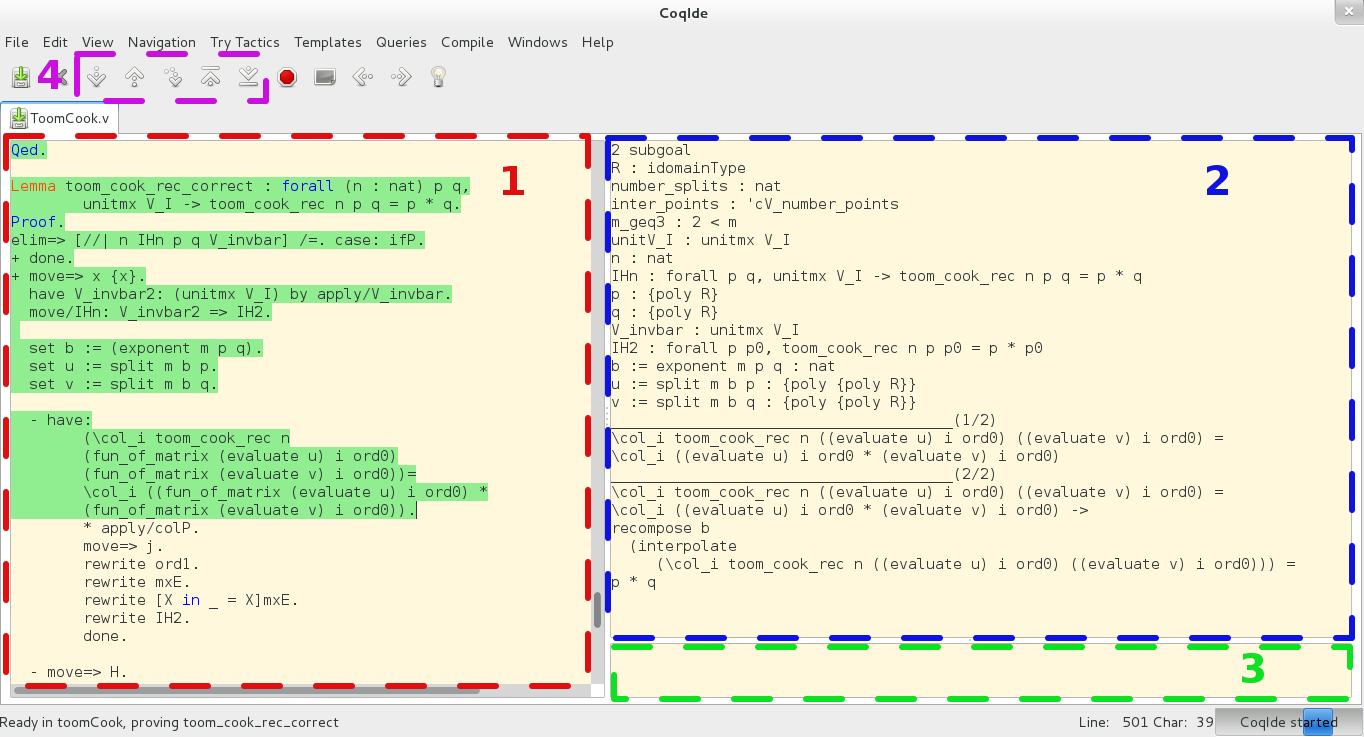
\includegraphics[width=\textwidth]{images/Overview}
  \caption[Översikt av \coq{} Ide]
   {Översikt av de olika delarna i \coq{} Ide}
  \label{fig:oversikt}
\end{figure}

Figur~\ref{fig:kontext} är är en förstoring av ruta 2 i Figur~\ref{fig:oversikt}
\begin{enumerate}
  \setcounter{enumi}{4}
\item Kontext, här visas vilka hypoteser och variabler som vi för tillfället
  har i beviset.
\item Mål, här visas vilka mål som ska uppnås. Det översta målet är det som
  användaren arbetar med för tillfället och det är det målet som kommer att
  påverkas av nästkommande taktik.
\end{enumerate}

\begin{figure}[H]
  \centering
  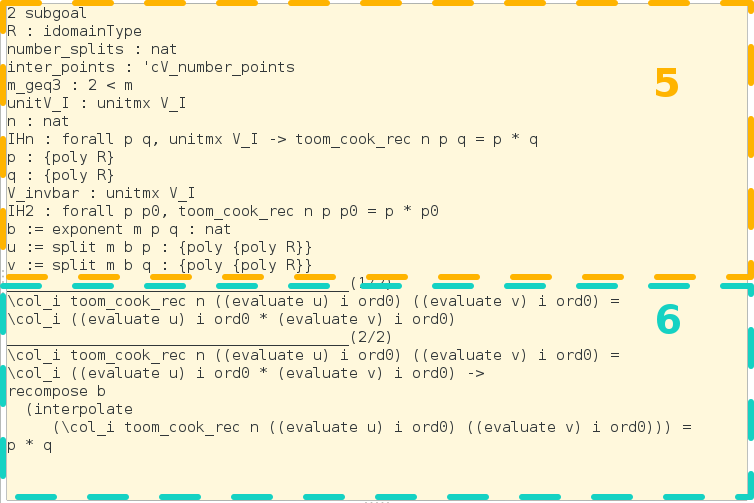
\includegraphics[width=150mm]{images/Kontext}
  \label{fig:kontext}
  \caption[Fönster för kontext och mål]
   {Textfönster för kontext och mål. Figuren visar en förstoring av ruta 2 i
    figur 4.1}
\end{figure}




\subsection{Evaluering av kod}
\coq{} är uppbyggt av satser där varje sats avslutas med en punkt. Koden
evalueras sedan en sats i taget och de delar av koden som har blivit evaluerade
markeras med en grön färg och det går inte längre att göra några ändringar i
dessa. Om man skulle vilja göra en ändring får man stega tillbaka
i programmet och göra ändringen. I följande sekvens av skärmdumpar visas
hur ett bevis

Figur~\ref{fig:bevis1} visar ett exempel på ett bevis för att följande påstående
är en tautologi. En tautologi är en logisk sats som alltid är sant oberoende av
sanningsvärdena på hypoteserna.


\begin{figure}[H]
  \centering
  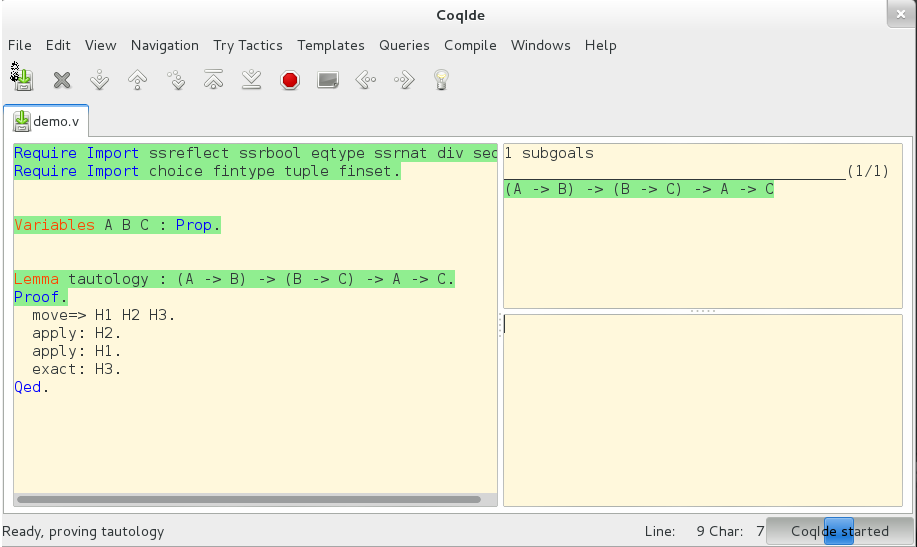
\includegraphics[width=100mm]{images/Proof_part1}
  \label{fig:bevis1}
  \caption[Exempel på bevis i \coq{}]
   {Exempel på ett bevis för en tautologi i \coq{}}
\end{figure}

Figurerna ~\ref{fig:bevis2} och ~\ref{fig:bevis3} visar den interaktiva
biten mellan \coq Ide och användaren. Notera hur mål och kontext uppdateras
efter att en taktik används och attden taktik som har evaluerats blir grönmarkerad.


\begin{figure}[H]
  \centering
  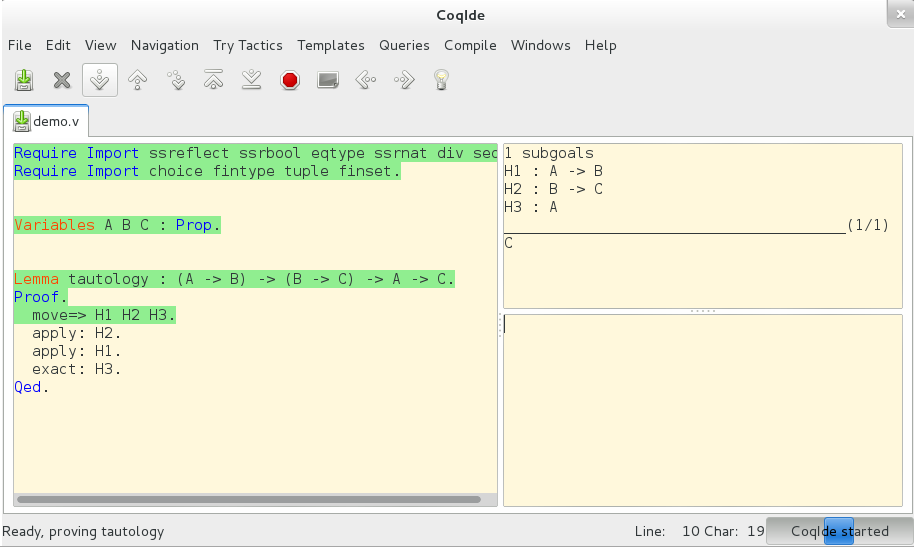
\includegraphics[width=150mm]{images/Proof_part2}
  \label{fig:bevis2}
  \caption[Bevis i \coq{} Ide]
   {Vi har nu flyttat hypoteserna (A $rightarrow$ B), (B $\rightarrow$ C) och A
    från målet till kontexten och med taktiken \C{move}}
\end{figure}

\begin{figure}[H]
  \centering
  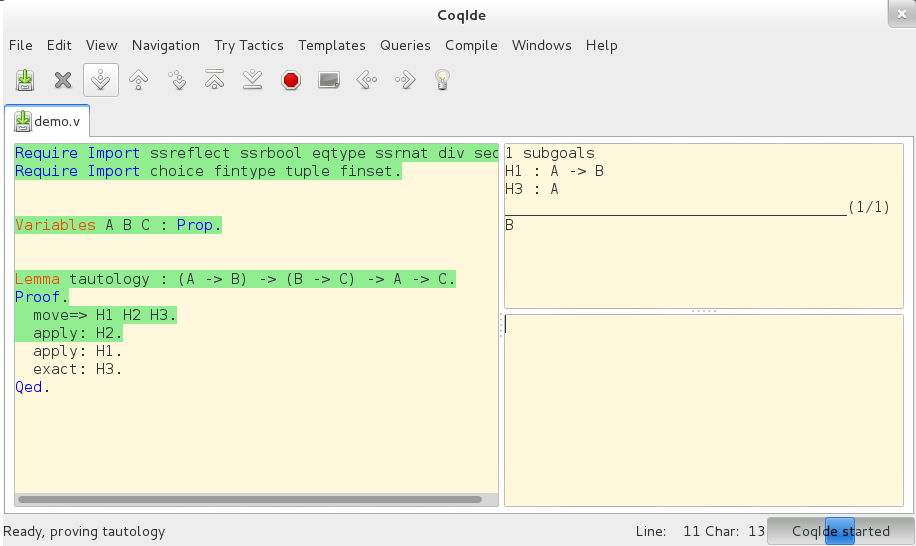
\includegraphics[width=150mm]{images/Proof_part3}
  \label{fig:bevis3}
  \caption[Bevis i \coq{} Ide]
   {Vi har nu använt oss av Hypotesen ($B \rightarrow C$) och vi
    kan se att målet nu har ändrat sig från C till B}
\end{figure}


\newpage
\chapter{Toom-Cook algoritmen}
Under senare år har några mycket långa och komplexa matematiska bevis
presenterats. Vissa bevis har också byggt på en mycket omfattande analys av
tusentals fall utförd av datorprogram. Det är mycket tidsödande och svårt, om
ens praktiskt möjligt att för hand kontrollera varje steg ett sådant bevis. Få
matematiker har tid, lust och den speciella kompetensen inom just det specifika
matematiska området som gör att de kan eller vill att ägna år åt att
kontrollera att ett sådant bevis är korrekt. Dessutom finns risken för att ett
fel i ett bevis ändå inte upptäcks vid kontroll om beviset är hundratals- eller
tusentals sidor långt\cite{harrison2008formal}.

Bevisassistenter, datorsystem för att formalisera och verifiera varje logiskt
steg i bevis, kan användas för att kontrollera bevis och därmed minska risken
för att de innehåller fel och öka tilltron till att de är korrekta.

Fyrfärgssatsen\cite{gonthier2008formal} och Feit-Thompsons
sats\cite{aschbacher2004status} är två exempel på satser vars bevis har
formaliserats och kontrollerats i bevisassistenter. Fyrfärgssatsen säger att
varje karta kan färgläggas med fyra färger så att inga regioner med gemensam
gräns får samma färg. Det ursprungliga beviset var över hundra sidor långt och
byggde också datorprogrammerad fallanalys av miljontals fall. Detta gjorde
beviset svårt att kontrollera och kontroversiellt. Beviset formaliserades och
verifierades i bevisassistenten \coq 1995.
%Lite mer om fyrfärgssatsen här?
%Lite mer om Odd order theorem här?

De verktyg som används vid formalisering och datorverifiering kan även användas
för att verifiera programkod. Formella metoder är således intressant för både
för programmerare och matematiker.
% Niclas: Den här meningen säger väldigt lite. Varför??
Dagens stora och komplexa programvaror skulle kunna utnyttja formella metoder.
%)
Det kan också vara användbart i kritiska system, till exempel medicinsk
utrustning, där det inte får bli fel eller i system som inte kan uppdateras i
efterhand som hårdvarunära mjukvara på ROM-minnen.

De mest använda metoderna idag för att kontrollera kod bygger på att testa om
koden ger korrekt resultat för olika indata. På detta sätt har man en chans att
upptäcka om koden innehåller fel, men det visar inte att koden saknar fel
eftersom det i många fall är omöjligt att testa alla kombinationer av indata.
% Niclas: + Svårt/Krävande att hitta kända resultat?
Formella metoder skulle i dessa fall kunna användas till att garantera
korrekthet hos koden.

Ett exempel på projekt för att verifiera kod är CompCert. Det utforskar
möjligheten att utveckla formellt bevisade kompilatorer. Anledningen att man
vill ha en formellt bevisad kompilator är att vid vissa optimeringar så kan
kompilatorn skapa buggar och beräkningsfel. Huvudresultatet av detta är en
fungerande C-kompilator som är bevisad i \coq och som stödjer hela ANSI C (som
är den första standardiserade versionen av C) med få
undantag\autocite{compcert}.

Matematisk programvara som MATLAB spelar en stor roll för beräkningar inom
forskning och industri och det finns därmed ett stort intresse av att de är
% Niclas: känns som det kan finnas bättre ord än buggfria
pålitliga. De är dock inte buggfria. Ett sätt att göra dem mer pålitliga skulle
vara att formalisera de ingående algoritmerna och visa att de är korrekt
implementerade\cite{denes2012refinement}.

Det här projektet går ut på att gruppdeltagarna ska lära sig formalisering med
bevisassistenten \coq och sedan formalisera och bevisa en matematisk algoritm,
\toom, i \coq.

\coq är en av flera avancerade bevisassistenter som det bedrivs aktiv forskning
om. Några andra är Agda, som utvecklats på Chalmers, Z3, som har utvecklats av
Microsoft och kan användas tillsammans med flera stora ickefunktionella språk
som Python, C och .NET och HOL-light, som används av Intel för att bevisa att
vissa hårdvarukomponenter fungerar korrekt och i det pågående projektet att
formalisera Keplers förmodan \cite{hales2008formal}.

\toom är en algoritm för att multiplicera heltal eller polynom. Den är
intressant eftersom den har en bättre asymptotisk tidskomplexitet än
polynommultiplikation utförd direkt enligt definitionen \footnote{För
definition av polynommultiplikation, se
appedix~\ref{appendix:matematikteori}.}, där man multiplicerar varje term i det
ena polynomet med varje term i det andra polynomet vilket har den asymptotiska
tidskomplexiteten $O\left(n^2\right)$\footnote{Funktionen $T(n)$ är $O(f(n))$
om det existerar konstanter $c > 0$ och $n_0 \geq 0$ så att $T(n) \leq c \cdot
f(n)$ för alla $n \geq n_0$.}, där n är graden på det största av de två
polynomen som skall multipliceras.

\section{Karatsuba}
\label{sec:karatsuba}
Karatsuba-algoritmen bygger på ett enkelt knep och visar tydligt varför vi kan
förbättra den asymptotiska tidskomplexiteten jämfört med naiv
polynommultiplikation. Säg att vi vill multiplicera polynomen $p$ och $q$. Vi
kan då dela upp polynomen $p$ och $q$ i två delar så att:
\begin{align*}
  p(x) &= p_0 + p_1 x^{\frac{n}{2}} \\
  q(x) &= q_0 + q_1 x^{\frac{n}{2}}
\end{align*}
Där $n$ är graden på det största polynomet. Multiplikationen kan då skrivas
som:
\begin{align*}
p(x)q(x) &= (p_0 + p_1 x^{\frac{n}{2}})(q_0 + q_1 x^{\frac{n}{2}}) \\
         &= p_0 q_0  + (q_0 p_1 +p_0 q_1 )  x^{\frac{n}{2}} + p_1 q_1  x^n
\end{align*}
Tricket i Karatsuba är följande enkla omskrivning som gör att vi blir av med en
multiplikation så att vi istället för fyra multiplikationer endast behöver tre
distinkta multiplikationer:
\begin{equation*}
  p_0 q_0 + ((p_1 + p_0)(q_1 + q_0) - p_1 q_1 - p_0 q_0)  x^{\frac{n}{2}} + p_1 q_1  x^n
\end{equation*}
Tidskomplexiteten för Karatsuba-algoritmen är då:
\begin{equation*}
  T(n) = 3 T(\lceil n/2\rceil) + cn + d
\end{equation*}
där $n$ är graden på det största polynomet och $c$ och $d$ är konstanter.

Genom att skriva ut rekurrensekvationen får vi att Karatsuba-algoritmen har den
asymptotiska tidskomplexiteten $\Ordo(n^{\log_2 3})$.

\section{Definition av Toom-Cook}
\label{sec:definition}
Det första steget i formaliseringen av Toom-Cook-algoritmen är en informell men
detaljerad definition och bevis av algoritmen och att den är korrekt. Detta
avsnitt är ägnat åt den. Versionen av algoritmen som presenteras bygger på den
i \cite{bodrato2007notes} och presentationen av den följer källans. För en
introduktion till integritetsområden och polynom, se appendix
\ref{appendix:matematikteori}.

Låt R vara ett integritetsområde och låt $p, q \in R[x]$, där
\begin{align*}
  p(x) &= a_0 + a_1 x + \cdots + a_n x^n, \\
  q(x) &= b_0 + b_1 x + \cdots + b_s x^s
\end{align*}
med $0 \leq s \leq n$.
I detta avsnitt definierar vi $\toomm (p, q)$, för naturliga tal $m \geq 3$,
som resultatet av algoritmen nedan.

\subsection{Gradkontroll}
\label{sec:gradkontroll}
Om $\grad p = n \leq 2$, låt $\toomm (p, q) = p \cdot q$, där $p\cdot q$
beräknas med naiv polynommultiplikation, annars gå vidare till steg
\ref{in:uppdelning}.

\subsection{Uppdelning}
\label{sec:uppdelning}
Låt
\begin{align}
  b &= \floor[\bigg]{\frac{1 + \grad p}{m}} + 1 = \floor[\bigg]{\frac{1 + n}{m}} + 1. \label{eq:b}
\intertext{För $f \in R[x]$ och}
  f &= q x^k + r
\intertext{med $q, r \in R[x]$ och $r = 0$ eller $\grad r \leq \grad x^k$, låt}
  f/x^k       &= q \label{eq:rdiv} \\
  f \modu x^k &= r. \label{eq:rmod}
\intertext{Nu definierar vi $u, v \in \left(R[x]\right)[y]$. Låt}
  u(y) &= u_0 + u_1 y + \cdots + u_{m-1} y^{m-1} \label{eq:u}
\intertext{där}
  u_k &= \left(p / x^{bk} \right) \modu x^b
\intertext{och}
  v(y)&=v_0 + v_1 y + \cdots + v_{m-1} y^{m-1} \label{eq:v}
\intertext{där}
  v_k &= \left(q / x^{bk} \right) \modu x^b
\end{align}
Vi vill alltså att $u(x^b)=p(x)$ och $v(x^b)=q(x)$.

\subsection{Evaluering}
\label{sec:evaluering}
Nu ska vi beräkna $w = u \cdot v$. Vi kommer göra detta genom interpolation i
steg~\ref{in:interpol}. Eftersom
\begin{align*}
 \grad w \leq \grad u + \grad v \leq m - 1 + m -1 = 2m-2 = d
\end{align*}
kan koefficienterna i $w$ bestämmas om vi vet värdet av $w$ i $d + 1$ skiljda
punkter. Vi evaluerar $w$ i punkterna $\alpha_0, ...,  \alpha_d$, där
$\alpha_i \in R$. För att göra det beräknar vi i detta steg först $u(\alpha_i)$
och $v(\alpha_i)$ genom matrismultiplikation. I nästa steg beräknas sen
$w(\alpha_i)=u(\alpha_i) \cdot v(\alpha_i)$. Låt

\begin{align*}
 V_e &=
\begin{pmatrix}
  \alpha_0^0 & \alpha_0^1 & \cdots & \alpha_0^{m-1} \\
  \vdots     & \vdots     & \ddots & \vdots         \\
  \alpha_d^0 & \alpha_d^1 & \cdots & \alpha_d^{m-1}
\end{pmatrix}.
\intertext{Då får vi}
  V_e \cdot
  \begin{pmatrix}
    u_0    \\
    \vdots \\
    u_{m-1}
  \end{pmatrix}
  &=
  \begin{pmatrix}
    u(\alpha_0) \\
    \vdots      \\
    u(\alpha_d)
  \end{pmatrix}
\end{align*}
och motsvarande för $v$.

\subsection{Rekursiv multiplikation}
\label{sec:rekursiv}
Vi beräknar $w(\alpha_i)=u(\alpha_i) \cdot v(\alpha_i)$ för i $= 0, \dots, d$
rekursivt genom att anropa Toom-Cook med $u(\alpha_i)$ och $v(\alpha_i)$ som
argument. Notera att $u(\alpha_i)$, $v(\alpha_i) \in R[x]$.

\subsection{Interpolation}
\label{sec:interpol}
Vi bestämmer koefficienterna i $w(y)=w_0 + w_1 y + \ldots + w_d y^d$ genom
interpolation. Vi vet värdet av $w(y) = u(y) \cdot v(y)$ i $d + 1$ punkter. Om

\begin{align}
  \label{eq:NAME3}
  V_I &=
  \begin{pmatrix}
    \alpha_0^0 & \alpha_0^1 & \cdots & \alpha_0^d \\
    \vdots     & \vdots     & \ddots & \vdots     \\
    \alpha_d^0 & \alpha_d^1 & \cdots & \alpha_d^d
  \end{pmatrix}
\intertext{så är}
  \label{eq:NAME4}
  V_I \cdot
  \begin{pmatrix}
    w_0    \\
    \vdots \\
    w_d
  \end{pmatrix}
  &=
  \begin{pmatrix}
    w(\alpha_0) \\
    \vdots      \\
    w(\alpha_d)
  \end{pmatrix}
\intertext{och därmed är}
  \label{eq:NAME5}
  \begin{pmatrix}
    w_0    \\
    \vdots \\
    w_d
  \end{pmatrix} &=
  V_I^{-1} \cdot
  \begin{pmatrix}
    w(\alpha_0) \\
    \vdots      \\
    w(\alpha_d)
  \end{pmatrix}
\intertext{förutsatt att $V_I$ är inverterbar. Detta är den om determinanten
$V_I$ är ett invertarbart elemet i $R$ [referens]. Eftersom $V_I$ är en
Vandermondematris så är}
  \label{eq:NAME6}
  \det V_I &= \prod_{0 \leq i < j \leq d} (\alpha_i - \alpha_j)
\end{align}

\subsection{Sammansättning}
\label{sec:sammansattning}
Vi får slutligen $p(x) \cdot q(x)$ genom att evaluera $w$ i $x^b$ eftersom
$w(x^b) = u(x^b) \cdot v(x^b)$.

\section{Exempel på Toom-3}
% Numrerade stycken som förra sektionen??

Antag att vi vill multiplicera två polynom $p, q \in
\Z_5[x]$\footnote{$\Z_5$ betecknar heltalen modulo 5.}. Vi
låter 0, 1, 2, 3 och 4 beteckna elementen i $\Z_5[x]$ och vi antar
\begin{align*}
  p(x) &= 4+x+3x^2+3x^3+4x^4 \\
  q(x) &= 1+2x+2x^2+x^3+3x^4
\end{align*}

\paragraph{Uppdelning}
Vårat $b$ i uppdelningssteget, som säger i hur stora delar vi ska dela upp
polynomen, ges av
\begin{equation*}
  b = \floor[\bigg]{\frac{1 + \mbox{grad p}}{\mbox{toom-instans}}} + 1 = \floor[\bigg]{\frac{1 + 4}{3}} + 1 = 2
\end{equation*}
Alltså delar vi polynomen vid potenser av $x$ som är multiplar av 2 och låter
delarna vara koefficienter i polynomen $u$ och $v$:
\begin{align*}
  u(y) &= (4+x)+(3 + 3x)y+ 4y^2 \\
  v(y) &= (1 + 2x)+ (2 + x)y + 3y^2
\end{align*}

\paragraph{Evaluering}
Om vi väljer evalueringspunkterna
\begin{equation*}
  0, 1, 2, 3, 4
\end{equation*}
så blir evalueringsmatrisen
\begin{equation*}
  V_e = \begin{pmatrix}
    0^0 & 0^1 & 0^2 \\
    1^0 & 1^1 & 1^2 \\
    2^0 & 2^1 & 2^2 \\
    3^0 & 3^1 & 3^2 \\
    4^0 & 4^1 & 4^2
  \end{pmatrix} =
  \begin{pmatrix}
    1 & 0 & 0 \\
    1 & 1 & 1 \\
    1 & 2 & 4 \\
    1 & 3 & 4 \\
    1 & 4 & 1
  \end{pmatrix}
\end{equation*}
Genom att multiplicera evalueringsmatrisen med vektorerna av koefficienter för
våra polynom $u$ och $v$ får vi vektorer med polynomens värden i
evalueringspunkterna.
\begin{equation*}
  \begin{pmatrix}
    u(0) \\
    u(1) \\
    u(2) \\
    u(3) \\
    u(4)
  \end{pmatrix} =
  \begin{pmatrix}
    1 & 0 & 0 \\
    1 & 1 & 1 \\
    1 & 2 & 4 \\
    1 & 3 & 4 \\
    1 & 4 & 1
  \end{pmatrix}
  \begin{pmatrix}
    4 + x \\
    3 + 3x \\
    4
  \end{pmatrix} =
  \begin{pmatrix}
    4 + x \\
    1 + 4x \\
    1 + 2x \\
    4 \\
    3x
  \end{pmatrix}
\end{equation*}
\begin{equation*}
  \begin{pmatrix}
    v(0) \\
    v(1) \\
    v(2) \\
    v(3) \\
    v(4)
  \end{pmatrix} =
  \begin{pmatrix}
    1 & 0 & 0 \\
    1 & 1 & 1 \\
    1 & 2 & 4 \\
    1 & 3 & 4 \\
    1 & 4 & 1
  \end{pmatrix}
  \begin{pmatrix}
    1 + 2x \\
    2 + x \\
    3
  \end{pmatrix} =
  \begin{pmatrix}
    1 + 2x \\
    1 + 3x \\
    2 + 4x \\
    4 \\
    2 + x
  \end{pmatrix}
\end{equation*}

\paragraph{Rekursiv multiplikation}
Genom att multiplicera $u$ och $v$ i de evaluerade punkterna rekursivt får vi
värdet i evalueringspunkterna av $u \cdot v = w$, där $w$ är det polynom som
skall interpoleras fram
\begin{equation*}
  \begin{pmatrix}
    w(0) \\
    w(1) \\
    w(2) \\
    w(3) \\
    w(4)
  \end{pmatrix} =
  \begin{pmatrix}
    u(0) \cdot v(0) \\
    u(1) \cdot v(1) \\
    u(2) \cdot v(2) \\
    u(3) \cdot v(3) \\
    u(4) \cdot v(4)
  \end{pmatrix} =
  \begin{pmatrix}
    4 + 4x + 2x^2 \\
    1 + 2x + 2x^2 \\
    2 + 3x + 3x^2 \\
    1 \\
    x + 3x^2
  \end{pmatrix}
\end{equation*}

\paragraph{Interpolation}
Vi vet att
\begin{equation*}
  V_I = \begin{pmatrix}
    0^0 & 0^1 & 0^2 & 0^3 & 0^4 \\
    1^0 & 1^1 & 1^2 & 1^3 & 1^4 \\
    2^0 & 2^1 & 2^2 & 2^3 & 2^4 \\
    3^0 & 3^1 & 3^2 & 3^3 & 3^4 \\
    4^0 & 4^1 & 4^2 & 4^3 & 4^4
  \end{pmatrix} =
  \begin{pmatrix}
    1 & 0 & 0 & 0 & 0 \\
    1 & 1 & 1 & 1 & 1 \\
    1 & 2 & 4 & 3 & 1 \\
    1 & 3 & 4 & 2 & 1 \\
    1 & 4 & 1 & 4 & 1
  \end{pmatrix}
\end{equation*}
och
\begin{equation*}
  V_I \cdot \begin{pmatrix}
    w_0 \\
    w_1 \\
    w_2 \\
    w_3 \\
    w_4
  \end{pmatrix} =
  \begin{pmatrix}
    w(0) \\
    w(1) \\
    w(2) \\
    w(3) \\
    w(4)
  \end{pmatrix}
\end{equation*}
där $w_0, \dots, w_4$ är koefficienterna i polynomet $w$. Determinanten till en
Vandermondematris kan räknas ut på följande sätt
\begin{align*}
 \det V_I &= (0-1)(0-2)(0-3)(0-4)(1-2)(1-3)(1-4)(2-3)(2-4)(3-4) \\
          &= 3  \\
          &\neq 0,
\end{align*}
så $V_I$ är inverterbar eftersom varje nollskiljt element i $\Z_5[x]$
har en multiplikativ invers. Vi får då koefficienterna till $w$ genom att
\begin{align*}
  \begin{pmatrix}
    w_0 \\
    w_1 \\
    w_2 \\
    w_3 \\
    w_4
  \end{pmatrix} & =
  V_I^{-1} \cdot \begin{pmatrix}
    w(0) \\
    w(1) \\
    w(2) \\
    w(3) \\
    w(4)
  \end{pmatrix} =
  \begin{pmatrix}
    1 & 0 & 0 & 0 & 0 \\
    0 & 4 & 2 & 3 & 1 \\
    0 & 4 & 1 & 1 & 4 \\
    0 & 4 & 3 & 2 & 1 \\
    4 & 4 & 4 & 4 & 4
  \end{pmatrix}
  \begin{pmatrix}
    w(0) \\
    w(1) \\
    w(2) \\
    w(3) \\
    w(4)
  \end{pmatrix} = \\
  &= \begin{pmatrix}
    4 + 4x + 2x^2 \\
    1 + 2x^2 \\
    2 + 3x^2 \\
    2 + 3x \\
    2
  \end{pmatrix}
\end{align*}
Då har vi
\begin{equation*}
  w(y) = (4 + 4x + 2x^2) + (1 + 2x^2)y + (2 + 3x^2)y^2 + (2 + 3x)y^3 + 2y^4
\end{equation*}

\paragraph{Sammansättning}
Produkten $p(x) \cdot q(x)$ får vi slutligen genom evaluera $w$ i
$x^b$, alltså i $x^2$.
\begin{align*}
  w(x^2) =& (4 + 4x + 2x^2) + (1 + 2x^2)x^2 + (2 + 3x^2)(x^2)^2 + (2 + 3x)(x^2)^3 + 2(x^2)^4 \\
         =& 4 + 4x + 2x^2 + x^2 + 2x^4 + 2x^4 + 3x^6 + 2x^6 + 3x^7 + 2x^8 \\
         =& 4 + 4x + 3x^2 + 4x^4 + 3x^7 + 2x^8
\end{align*}

\section{Informellt bevis av Toom-Cook}
\label{informhuvudbevis}
I detta stycke visar vi att för $p, q \in R[x]$ så är
$p \cdot q = Toom-Cook (p, q)$. Vi gör detta med hjälp av två lemman, vars bevis
kommer efter beviset av~\ref{prop:1}.

\begin{proposition}
  \label{prop:1}
  Antag att $R$ är ett integritetsområde och att $p, q \in R[x]$. Om det finns
  $\alpha_0, \dots, \alpha_{2m-2} \in R$ så att $\prod_{0 \leq i < j \leq d}
  (\alpha_i - \alpha_j)$ är inverterbar i $R$, så är med dessa punkter som
  interpolationspunkter

  \begin{equation}
    \label{eq:name7}
    Toom-Cook (p, q) =  p \cdot q.
  \end{equation}
\end{proposition}

\begin{proof}
Vi visar propositionen med induktion över $\grad p$.

\paragraph{Basfall.}
När $n = \grad p \leq 2$ så gäller (\ref{eq:name7}) enligt steg
\ref{in:gradkontroll} i algoritmen eftersom att vi räknar ut produkt direkt.

\paragraph{Induktionssteg.}
\label{in:induktion}
Antag att $p, q \in R[x]$, där
\begin{align*}
  p(x) &= a_0 + a_1 x + \cdots + a_n x^n, \\
  q(x) &= b_0 + b_1 x + \cdots + b_s x^s
\end{align*}
med $0 \leq s \leq n$.

\bigskip\noindent
Antag också att $n > 2$ och att $Toom-Cook (f, g) =  f \cdot g$ gäller för polynom
av grad mindre än $n$. Eftersom $n > 2$ så går vi vidare till steg
\ref{in:gradkontroll} i algoritmen och skapar $u$ och $v$ från $p$ och $q$. När
detta är gjort evaluerar vi i steg 3 $u$ och $v$ i punkterna $\alpha_0, \dots,
\alpha_{2m-2}$ genom att multiplicera vektorn av deras koefficienter med
evalueringsmatrisen. I steg~\ref{in:rekursiv} anropar vi Toom-Cook igen, nu med
argumenten $u(\alpha_i) \cdot v(\alpha_i)$ för $i = 0, \ldots , 2m-2$. Dessa är
polynom i $R[x]$. Eftersom $\grad u(\alpha_i)$, $\grad v(\alpha_i) < n$ enligt
lemma~\ref{lemma:1} så är $Toom-Cook (u(\alpha_i), v(\alpha_i)) = u(\alpha_i) \cdot
v(\alpha_i)$ enligt induktionsantagnandet. I steg~\ref{in:interpol} skall vi
bestämma koefficienterna i $w(y)=u(y) \cdot v(y)$. Detta gör vi genom att lösa
matrisekvationen (\ref{eq:NAME4}). Eftersom interpolationsmatrisen $V_I$ enligt
antagande är inverterbar så ges koefficienterna entydigt av (\ref{eq:NAME5}). I
steg~\ref{in:sammansattning} evaluerar vi $w(y)=u(y) \cdot v(y)$ i $x^b$. Lemma
\ref{lemma:2} ger att $u(x^b)=p(x)$ och att $v(x^b)=q(x)$. Då $w(y)=u(y) \cdot
v(y)$ så är $w(x^b)=u(x^b) \cdot v(x^b)=p(x) \cdot q(x)$.
\end{proof}

\begin{lemma}
  \label{lemma:1}
  Antag att $p(x) \in R[x]$ och att $\grad p \geq 2$. Antag också att $u(y)$ är
  definierad enligt steg~\ref{in:uppdelning}, uppdelning, i algoritmen och att
  $\alpha \in R$. Då är $\grad u(\alpha) < \grad p$.
\end{lemma}
\begin{proof}
  Eftersom $\alpha \in R$ så är
  \begin{align*}
    \grad u(\alpha) &= \grad (u_0 + u_1 \alpha + ... + u_{m-1}\alpha^{m-1}) = \max \grad u_k,
  \end{align*}
  där $k={0,1,...,m-1}$.

  \bigskip\noindent
  $u_k = p(x)/x^{k b} \modu x^b$, så enligt definition av mod så är $\grad u_k
  < b$. Nu återstår att visa att $b < \grad p = n$. Vi har definierat $b =
  \floor[\big]{\frac{1 + n}{m}} + 1$. Om $n \geq 2$ och $m \geq 3$ så är
  \begin{align*}
    n-b &= n - \left( \floor[\bigg]{\frac{1 + n}{m}} + 1 \right) \geq \frac{nm-n-m-1}{m} \geq 0,
  \end{align*}
  så $\grad u(\alpha) < b \leq \grad p(x) = n$.
\end{proof}

\begin{lemma}
  \label{lemma:2}
  Antag att $p(x) \in R[x]$ och att $b$ och $u(y)$ är definierade som i steg 2
  i algoritmen. Då är $u(x^b)=p(x)$.
\end{lemma}
\begin{proof}
  Vi har att
  \begin{align*}
    u(x^b) &= \sum_{i = 0}^{m-1} p(x)/x^{bi} (\modu x^b) x^{bi} \\
           &= \sum_{i = 0}^{m-2} p(x)/x^{bi} (\modu x^b) x^{bi} + p(x)/x^{b(m-1)} (\modu x^b) x^{b (m-1)}.
  \end{align*}
  \paragraph{Påstående 1.} Den sista termen i $u(x^b)$ kan skrivas om till
  $p(x)/x^{b (m-1)} x^{b (m-1)}$ eftersom $\grad p - b (m-1) < b$.

  Med $\grad p = n$ och $b = \floor[\big]{\frac{1 + n}{m}} + 1$ har vi att
  \begin{align*}
    b - (n - b(m-1)) &= m b - n \\
                     &= m \left( \floor[\bigg]{\frac{1 + n}{m}} + 1 \right) - n \\
                     &= m \left( \frac{1 + n}{m} - \left\{ \frac{1 + n}{m} \right\} \right) + m - n \\
                     &= 1 + n - m \left\{ \frac{1 + n}{m} \right\} + m - n \\
                     &= 1 + m \left( 1 - \left\{ \frac{1 + n}{m} \right\} \right) > 0
  \end{align*}
  eftersom $0 < 1 - \{ x \} \leq 1$ för alla reella tal $x$
  \footnote{$\{x\}$ betecknar $x-\lfloor x \rfloor$. Se \cite{graham1989concrete}.}.
  Graden av $p(x)/x^{b(m-1)}$ är $\max \{n - b(m-1),0\}$ som är mindre än $b$,
  och därmed är $p(x)/x^{b(m-1)}  \modu x^b = p(x)/x^{b(m-1)}$, vilket visar
  Påstående 1. Så
  \begin{align*}
    u(x^b) &= \sum_{i = 0}^{m-2} p(x)/x^{bi} (\modu x^b) x^{bi} + p(x)/x^{b(m-1)} x^{b(m-1)}.
  \end{align*}
  För alla polynom $a(x)$ gäller att
  \begin{align}
    a(x) = a(x) \modu x^b + \left(a(x)/x^b\right) x^b \label{eq:name8}
  \end{align}
  då $a(x) \modu x^b$ och $p(x)/x^{b}$ är resten respektive kvoten vid division
  med $x^b$. Så om vi kan visa att $u(x^b) = p(x) \modu x^b + p(x)/x^{b} x^{b}$
  så är $u(x^b) = p(x)$. Och om sedan
  \begin{align}
    \sum_{i = 0}^{k} p(x)/x^{bi}  (\modu x^b) x^{bi} + (p(x)/x^{b(k + 1)})  x^{b(k + 1)} = \label{eq:name9} \\
    \sum_{i = 0}^{k-1} p(x)/x^{bi}  (\modu x^b) x^{bi} + (p(x)/x^{b k})  x^{b k} \label{eq:name10}
  \end{align}
  för $k \geq 1$ så ger induktion över $k$ att $u(x^b) =  p(x)$. Nu återstår
  alltså bara att visa att (\ref{eq:name9}) = (\ref{eq:name10}).

  \begin{align*}
    \sum_{i = 0}^{k} p(x)/x^{bi} (\modu x^b) x^{bi} &+ p(x)/x^{b(k + 1)}  x^{b(k + 1)} =\\
    \sum_{i = 0}^{k-1} p(x)/x^{bi} (\modu x^b) x^{bi} &+
    \left(p(x)/x^{b k} \modu x^b\right) x^{b k} + \left(p(x)/x^{b(k + 1)}\right)  x^{b(k + 1)} = \\
    \sum_{i = 0}^{k-1} p(x)/x^{bi} (\modu x^b) x^{bi} &+
    \left(p(x)/x^{b k} \modu x^b + \left(p(x)/x^{b(k + 1)}\right)  x^b \right) x^{b k} = \\
    \sum_{i = 0}^{k-1} p(x)/x^{bi} (\modu x^b) x^{bi} &+
    (p(x)/x^{b k} \modu x^b + ((p(x)/x^{b k})/x^b)  x^b) x^{b k} =
    \tag{på grund av (\ref{eq:name8})}\\
    \sum_{i = 0}^{k-1} p(x)/x^{bi}  (\modu x^b) x^{bi} &+ (p(x)/x^{b k}) x^{b k}
  \end{align*}
\end{proof}


\newpage
\chapter{Formell implementation av Toom-Cook}
\section{Implementation av Toom-Cook i \coq{}}
\label{sec:formellimplementation}
I det här avsnittet förklaras hur Toom-Cook-algoritmen är implementerad i \ssr{}
och hur den överrenstämmer med pappersdefinitionen av algoritmen. Hela
implementation ligger som ett appendix~\ref{appendix:matematikteori}.

\subsection{Definitioner}
Algoritmen är implementerad med en rad små funktioner och sedan en rekursiv
del. Till en början kommer alltså många variabler, definitioner och antaganden
radas upp, som vi har försökt att ge så självförklarande namn som möjligt.

\begin{lstlisting}
Variable R : idomainType.
Implicit Types p q : {poly R}.
\end{lstlisting}

De här raderna säger att \C{R} betecknar ett integritetsområde och att \C{p}
och \C{q} är polynom i detta område.

\begin{lstlisting}
Variable number_splits : nat.
Definition m : nat := number_splits.
Definition number_points := (2 * m) .-1.
\end{lstlisting}

Här definieras variabler av typen nat, naturliga tal\footnote{I \coq{} och \ssr{}
är 0 inkluderad bland de naturliga talen}, vars värde beror på antalet splittar
som görs av polynomet. Precis som i pappersalgoritmen är \C{m} variabeln från
Toom-Cook-m och \C{number_points} är antalet interpolationspunkter.

\begin{lstlisting}
Variable inter_points : 'cV[{poly R}]_(number_points).
\end{lstlisting}

Vi låter \C{inter_points} beteckna en kolonnvektor vars element tillhör $R[x]$,
vilket faktiskt skiljer sig från pappersalgoritmen. Det var avgörande för
pappersalogritmen att punkterna tillhörde $R$ för att graden garanterat skulle
avta vilket ledde till att induktionsantagandet över graden kunde appliceras,
se avsnitt~\ref{sec:induktion}, men i beviset i\ssr{} görs induktion över en annan
variabel så det problemet uppstår aldrig. Algoritmen blir dock snabbare om
interpolationspunkterna tillhör $R$ eller är av låg grad i $R[x]$, se
avsnitt~\ref{def}.

\begin{lstlisting}
Hypothesis m_neq_0 : 0 < m.
\end{lstlisting}

I pappersalgoritmen har vi som antagande att \C{m} är större än två och här kan
vi återigen uttnyttja att induktionen görs över en annan variabel än graden, då
kommer vi runt problemet i lemma (\ref{lemma:1}), och kan vi få ner kravet till
att \C{m} måste vara större än noll.

\begin{lstlisting}
Definition V_e : 'M[{poly R}]_(number_points, m) :=
  \matrix_(i < number_points, j < m) ((inter_points i 0))^+j.
\end{lstlisting}

Här definieras evalueringsmatrisen \C{V_e}. Den ska ha dimension
\C{number_points} x \C{m} med element som tillhör $R[x]$. Argumentet \C{(i <
number_points, j < m)} säger just att matrisen är av dimensionen
\C{number_points} x \C{m}. Det andra argumentet \C{((inter_points i 0))^+j}
bestämmer vilket element som ska vara på plats \C{(i,j)} i matrisen, vilket i
det här fallet är det \C{i}:te elementet ur kolonnvektorn \C{inter_points}
upphöjt i \C{j}, vilket då blir en Vandermondematris.

\begin{lstlisting}
Definition V_I : 'M[{poly R}]_(number_points) :=
  \matrix_(i < number_points, j < number_points) ((inter_points i 0))^+j.
\end{lstlisting}

Här definieras interpolationsmatrisen på motsvarade sätt som
evalueringsmatrisen, skillnaden är att det blir en matris av dimension
\C{number_points} x \C{number_points} istället.

\begin{lstlisting}
Definition exponent (m: nat) p q : nat :=
  (maxn (divn (size p) m) (divn (size q) m)).+1.
\end{lstlisting}

Här definieras \C{exponent} som tar ett naturligt tal \C{m} som inparameter och
ger ett naturligt tal som utparameter. Om inparametern har värdet av m i
Toom-Cook-m så motsvarar det här b i pappers algoritmen, se ekvationen
(\ref{eq:b}), eftersom \C{size} tar graden av polynomet + 1, \C{divn} är
heltalsdivision och \C{maxn} tar fram det största av två tal. Funktionerna
\C{size}, \C{divn} och \C{maxn} är implementerade i \ssr{} bibliotek.

\begin{lstlisting}
Definition split (n b: nat) p : {poly {poly R}} :=
  \poly_(i < n) rmodp (rdivp p 'X^(i * b)) 'X^b.
\end{lstlisting}

\C{split} tar två naturliga tal som inparametrar och returnerar ett polynom som
polynom som tillhör $R[x][y]$. De två funktionerna \C{rmodp} och \C{rdivp} är
redan implementerade i \ssr{} bibliotek och motsvarar exakt vår definition av
modulusräkning och polynomdivision, se ekvationerna (\ref{eq:rmod}) och
(\ref{eq:rdiv}). Funktionerna \C{\\poly_(i<n}, \C{rmodp} och \C{rdivp} bildar
tillsammans motsvarande polynom
$u(y)=(p/x^0\;mod\;x^b)y^0+...+(p/x^{(n-1)b}\;mod\;x^b)y^{n-1}$ där \C{n} och
\C{b} är inparametrarna.

\begin{lstlisting}
Definition evaluate (u: {poly {poly R}}) : 'cV[{poly R}]_(number_points) :=
  V_e *m (poly_rV u)^T.
Definition interpolate (u: 'cV[{poly R}]_(number_points)) : {poly {poly R}} :=
  rVpoly (invmx V_I *m u)^T.
\end{lstlisting}

Här definieras själva matrismultiplikationerna, se ekvation (\ref{align:eval})
och (\ref{eq:NAME5}). Funktionen \C{poly_rV} gör ett polynom \C{u}, som
tillhör $R[x][y]$, till en radvektor där varje koefficient och respektive
potens av polynoment placeras in på respektive position i radvektorn. Vektorn
transponeras för att kunna multipliceras med evalueringsmatrisen.

\begin{lstlisting}
Definition recompose (b: nat) (w: {poly {poly R}}) : {poly R} :=
  w.['X^b].
\end{lstlisting}

Här sker evalueringen av \C{w} i $x^b$ där \C{b} är en inparametern.

\subsection{Rekusiv del}

Fjärde steget i Toom-Cook-algoritmen. se avsnitt~\ref{sec:rekursiv},  är en rekusiv del och
rekusiv del och därmed behövs en rekusiv funktion, nämligen Fixpoint, för att
kunna stega igenom hela algoritmen. I pappersalgoritmen slutar rekusionen när
graden har blivit tillräckligt låg och då utförs direktmultiplikation. \coq{}
behöver få bevisat att rekusionen terminar så istället för att visa att graden
sjunker för varje steg så skickas ett naturligt tal \C{n}, som inparameter, som
minskar vid varje rekusion och slutar när \C{n} är lika med noll eller när
graden har blivit mindre än 2 på någotdera av polynomen, och då utförs direkt
multiplikation. Så för att visa att Toom-Cook-algoritmen fungerar måste
algoritmen fungera för alla \C{n} eftersom fixpoint-funktion bara kommer motsvara
Toom-Cook om \C{n} är tillräckligt stort, ty tillräckligt många rekursiva anrop
måste göras.

% Lite skumt skrivet
Funktionen match kollar om \C{n} är lika med 0 i så fall retunera \C{p} gånger
\C{q} eller om \C{n} är en efterföljare till något tal.


\begin{lstlisting}
Fixpoint toom_cook_rec (n: nat) p q : {poly R} :=
  match n with
  | 0%N => p * q
  | n'.+1 => if (size p <= 2) || (size q <= 2) then p * q else
        let b := exponent m p q in
        let u := split m b p in
        let v := split m b q in
        let u_a := evaluate u in
        let v_a:= evaluate v in
        let w_a := \col_i toom_cook_rec n' (u_a i 0) (v_a i 0) in
        let w := interpolate w_a
         in recompose b w
  end.
\end{lstlisting}

\begin{lstlisting}
| 0%N => p * q
\end{lstlisting}

Om en \C{n} är lika med noll så sker direktmultiplikation mellan polynomen.

\begin{lstlisting}
| n'.+1 => if (size p <= 2) || (size q <= 2) then p * q else
\end{lstlisting}

Om en \C{n} då är en efterföljare till ett naturligt tal, med andra ord skiljt
från noll, då sker gradkontrollen, se avsnitt~\ref{sec:gradkontroll}, och direkt
multiplikation sker. Om båda polynomen är av högre grad än två så stegar vi
vidare i algoritmen.

\begin{lstlisting}
let b := exponent m p q in
\end{lstlisting}

% Lite svårt att förstå. Man måste tänka igenom texten ettpar gånger
Här låter vi \C{b} få värdet från funktionen \C{exponent} vilket blir det
värdet som i pappersalgoritmen, se ekvationen (\ref{eq:b}), eftersom \C{m} är
antalet splittar, \C{p} och \C{q} är polynomen i $R[x]$.

\begin{lstlisting}
let u := split m b p in
let v := split m b q in
\end{lstlisting}

Här låter vi \C{u} och \C{v} vara de polynom som funktionen \C{split}
retunerar, som tillhör $R[x][y]$. Inparametern \C{m} är antalet splittar, \C{b}
bestämdes i raden före, \C{p} och \C{q} är återigen polynomen i $R[x]$ så blir \C{u}
\C{u} och \C{v} motsvarande u och v i pappersalgoritmen, se ekvationerna
(\ref{eq:u}) och (\ref{eq:v}). Det här motsvarar alltså andra steget i
algoritmen, se avsnitt (\ref{sec:uppdelning}).

\begin{lstlisting}
let u_a := evaluate u in
let v_a:= evaluate v in
\end{lstlisting}

Här sker tredje steget i alogritmen, nämligen matrismultiplikationen mellan
evalueringsmatrisen och de olika polynomen \C{u} och \C{v} som representeras
som vektorer i evalueringen.

\begin{lstlisting}
let w_a := \col_i toom_cook_rec n' (u_a i 0) (v_a i 0) in
\end{lstlisting}

Det här motsvarar fjärde steget i algoritmen, rekusionens multiplikationen. Då
anropar funktionen \C{Fixpoint} sig själv med \C{n'} som inparameter, vilket
har värdet n-1, och de två polynomen \C{u} och \C{v}, representerade som
kolonnvektor, från evalueringssteget som inparametrar. \C{\\col_i}, \C{(u_a i
0)} tillsammans med \C{(v_a i 0)} beskriver att det \C{i}:te elementet ur
vardera vektor ska genomgå rekusionen och sedan presenteras på plats \C{i} i
kolonnvektorn \C{w_a}.

\begin{lstlisting}
let w := interpolate w_a
in recompose b w
\end{lstlisting}

När rekusionssteget är klart så sker interpolerationssteget, se avsnitt
\ref{sec:interpol}, där inversen av interpolationsmatrisen multipliceras med
kolonnvektorn \C{w_a} och retunerar polynomet \C{w} som är produkten av
polynomen u och v. Slutligen sker sammansättningen, se avsnitt
\ref{sec:sammansattning}, där \C{b} anger vilken exponent x får som evalueras in
polynomet \C{w} och därmed har vi produkten av polynomen \C{p} och \C{q}.

\section{Formellt bevis av Toom-Cook}
\label{sec:formellbevis}
Det här avsnittet presenterar det formella beviset för att den implementerade
algoritmen är korrekt. Många av detaljerna i beviset är rent tekniska och
förklaras inte närmare. Jämförelser görs med det informella beviset i avsnitt
\ref{sec:informhuvudbevis}. De viktigaste taktikerna som används förklaras under
bevisets gång. Variablerna \C{p} och \C{q} betecknar genomgående polynom över
ett integritetsområde.

I beviset används när så är möjligt redan tidigare bevisade resultat från \ssr{}
s bibliotek. En lång rad lemman om bland annat grundläggande egenskaper hos
polynom, naturliga tal, matriser och summor finns tillgängliga.

Det formella bevisets struktur är modellerad efter det informella bevisets i
avsnitt~\ref{sec:informhuvudbevis}, med ett huvudbevis som bygger på ett
flertal lemman. De formella lemmorna är dock många fler än de för det
informella beviset, 15 jämfört med två. Det beror delvis på att påståenden
delats upp i flera delpåståenden för att underlätta arbetsfördelningen inom
gruppen, men i första hand på att resonemangssteg som i det informella beviset
ses som så triviala att de inte ens nämns också måste visas när beviset
formaliseras. En ytterligare anledning är att det är är lättare att göra
omskrivningar och slutledningssteg på mindre delpåståenden separat. Ett 50-tal
mer generella lemman ur \ssr{}-biblioteket och ett par lemman som byggde på
grundläggande egenskaper hos polynomdivision som gick utanför projektets
avgränsningar och som tillhandahållits av projektets handledare, Anders
Mörtberg, har används i huvudbeviset och i beviset av lemmorna.

Nedan beskrivs huvudbeviset rad för rad, och därefter beskrivs några av de mer
intressanta lemmorna utan bevis.

\subsection{Huvudbeviset}
Detta är den formella motsvarigheten till prop~\ref{prop:1} för den
implementerade algoritmen. Eftersom \C{toom_cook} bara utvärderar
\C{toom_cook_rec} med ett visst argument så beror dess korrekthet helt på
följande sats, som säger att \C{toom_cook_rec} är korrekt:
\begin{lstlisting}
Lemma toom_cook_rec_correct : forall (n : nat) p q,
  unitmx V_I -> toom_cook_rec n p q = p * q.
\end{lstlisting}
När detta lemma är bevisat följer \C{toom_cook_correct} direkt:
\begin{lstlisting}
Lemma toom_cook_correct : forall p q,
   toom_cook p q = p * q.
 Proof. move=> p q. by apply: toom_cook_rec_correct. Qed.
\end{lstlisting}
Det formella beviset för att den rekursiva delen av algoritmen är korrekt har
en struktur som liknar beviset av prop~\ref{prop:1}.
% Konstig mening svårt att förstå vad som menas:
Den största skillnaden att induktionen i det formella fallet görs över antalet
rekursiva anrop av algoritmen i stället för att som i beviset av
prop~\ref{prop:1} görar över graden av de polynom som multipliceras. Det beror
på att den rekursiva delen av den implementerade algoritmen \C{toom_cook_rec}
är definierad med en oberoende variabel n, så som beskrivits i
\ref{section:formrec}. I stället för att induktionen som i det informella
beviset bygger på att graden av de polynom som Toom-Cook anropas med minskar
vid rekursiva anrop av algoritmen bygger den på att variabeln n minskas vid
rekursiva anrop. I båda fallen innebär dock induktionsantagandet att vi antar
att algoritmen fungerar korrekt för nästa lägre rekursiva anrop.
%Det nästa lägre anrop, finns det något bättre sätt att säga det här?
Den andra stora skillnaden mellan det informella och det formella beviset är
att många tekniska detaljer, som kan tas för givna i ett informellt bevis måste
visas explicit. Dessutom måste hänsyn tas till hur matriser och polynom är
representerade i \ssr{}.

Här nedan ges den fullständiga programkoden för att beviset av att den
rekursiva delen av algoritmen är korrekt, givet vissa lemman:
\lstset{numbers=left}
\begin{lstlisting}[escapeinside={@}{@}]
@\label{lst:rad1}@Lemma toom_cook_rec_correct : forall (n : nat) p q,
@\label{lst:rad2}@  unitmx V_I -> toom_cook_rec n p q = p * q.
@\label{lst:rad3}@Proof.
@\label{lst:rad4}@  elim=> [ // | n IHn p q V_inver] /=.
@\label{lst:rad5}@  set b := exponent m p q.
  set u := split m b p.
@\label{lst:rad7}@  set v := split m b q.
  case: ifP => [ // | _ ].
    have ->:
      \col_i toom_cook_rec n ((evaluate u) i 0) ((evaluate v) i 0) = \col_i ((evaluate u) i 0 * (evaluate v) i 0).
        apply/colP => j.
        by rewrite mxE [X in _ = X]mxE (IH2 _ _ V_inver).
      rewrite 2!matrix_evaluation.
      have ->:
        \col_i ((\col_j u.[inter_points j 0]) i 0 * (\col_j v.[inter_points j 0]) i 0) = \col_i (u * v).[(inter_points i 0)].
           apply/colP => k.
           by rewrite 4!mxE -hornerM.
      rewrite toom_cook_interpol //; last by apply: size_split_mul.
      rewrite /recompose hornerM.
      rewrite 2?recompose_split //.
      rewrite /b exponentC.
      by apply: exp_m_degree.
      by apply: exp_m_degree.
Qed.
\end{lstlisting}
\lstset{numbers=none}
På rad~\ref{lst:rad1} och \ref{lst:rad2} och formuleras lemmat och på rad
\ref{lst:rad3} anges att beviset startar genom \C{Proof}. Rad \ref{lst:rad4}
anger med \C{elim=>} att beviset kommer göras med induktion över den variabel
som står först i lemmat, \C{n}. Basfallet är trivialt precis som i
prop~\ref{prop:1} eftersom \C{toom_cook_rec} är vanlig multiplikation när
\C{n}$=0$ och delmålet det utgör avslutas direkt med hjälp av \C{//}. Till
höger om \C{|} ges instruktioner till induktionssteget. Variabeln \C{n'} där
\C{n' + 1}  = \C{n}, för det \C{n} som induktionen görs över instansieras.
Induktionsantagnandet \C{IHn}, polynomen \C{p} och \C{q} och antagandet
\C{V_inver} om att interpolationsmatrisen är inverterbar instansieras också.
Till sist skriver \C{/=} om målet genom att utveckla definitionen av
\C{toom_cook_rec}.

Raderna \ref{lst:rad5} till \ref{lst:rad7} sätter kortare beteckningar på några
av uttrycken i målet för att öka bevisets läslighet. Efter det har målet och
kontexten blivit:
\begin{lstlisting}
n' : nat
IHn : forall p q, unitmx V_I -> toom_cook_rec n' p q = p * q
p : {poly R}
q : {poly R}
V_inver : unitmx V_I
b := exponent m p q : nat
u := split m b p : {poly {poly R}}
v := split m b q : {poly {poly R}}
______________________________________(1/1)
(if (size p <= 2) || (size q <= 2)
  then p * q
  else
   recompose b
     (interpolate
       (\col_i
         toom_cook_rec n' ((evaluate u) i 0) ((evaluate v) i 0)))) =
p * q
\end{lstlisting}
Nästa steg är sedan att skriva om målet så att vi kan använda
induktionsantagandet \C{IHn}.

Först tar vi hand om \C{if ... then ... else} - uttrycket i vänsterledet.
Det säger att vänsterledet är lika med \C{p * q} om graden
av \C{p} eller \C{q} är mindre än 2 (eftersom multiplikation i algoritmen
då utförs direkt enligt definitionen) och annars
lika med det mer komplicerade uttrycket som står efter \C{else}. Dessa två
uttryck skulle motsvarat basfallet och induktionssteget om induktionen hade
gjorts över graden av p och q, som i prop~\ref{prop:1}.

Nu görs i stället på
rad~\ref{lst:rad8} med \C{ifP} en falluppdelning över \C{if ... then ... else}-uttrycket
som inte ger oss något nytt induktionsantagende.
I det första fallet när \C{(size p <= 2) || (size q <= 2)} är höger- och
vänsterled i målet trivialt lika
och löses liksom det triviala målet på rad \ref{lst:rad4} direkt med \C{//}.
När det är gjort är målet:
\begin{lstlisting}
recompose b
  (interpolate
    (\col_i
      toom_cook_rec n' ((evaluate u) i 0) ((evaluate v) i 0))) =
 p * q
\end{lstlisting}
och vi vill använda induktionsantagandet
\begin{lstlisting}
IHn : forall p q, unitmx V_I -> toom_cook_rec n' p q = p * q
\end{lstlisting}
tillsammans med antagandet \C{V_inver} om att \C{V_I} är inverterbar för att
skriva om
\begin{lstlisting}
toom_cook_rec n' ((evaluate u) i 0) ((evaluate v) i 0)
\end{lstlisting}
till \C{((evaluate u) i 0) * ((evaluate v) i 0)} inne i kolonnvektorn
\begin{lstlisting}
\col_i toom_cook_rec n' ((evaluate u) i 0)((evaluate v) i 0)
\end{lstlisting}
Eftersom definitionen \C{\\col_i} är låst för beräkning och uttrycket beror av
indexet \C{i} i kolonnvektorn kan vi inte direkt skriva om uttrycket, se
avsnitt~\ref{ssreflect}. Så för att kunna göra det öppnar vi ett nytt delmål
med taktiken \C{have} på rad~\ref{lst:rad9} där vi bara arbetar med denna del av
vänsterledet. Där använder vi på rad~\ref{lst:rad12} lemmat \C{colP} som låter oss visa
att två vektorer är lika genom att visa att elementen på motsvarande platser är
lika i båda vektorerna. (Då vektorer är implementerade i \ssr{} som funktioner
från mängden av index i vektorn $\{0, \ldots , k\}$ till mängden av element i
vektorn säger lemmat mer specifikt att två vektorer är lika om de extensionellt
sett är samma funktion, dvs om de antar samma värden för samma argument.) På
rad~\ref{lst:rad13} kan vi sedan slutligen visa att uttrycket i vänsterledet i
\C{have}-satsen är lika med uttrycket i högerledet i \C{have}-satsen med hjälp
av induktionshypotesen. Därefter kan det ursprungliga målet skrivas om till: då
blivit:
\begin{lstlisting}
recompose b
  (interpolate (\col_i ((evaluate u) i 0 * (evaluate v) i 0))) =
    p * q
\end{lstlisting}

Det återstår nu att visa tre saker: För det första att evalueringsfunktionen
\C{evaluate} faktiskt ger tillbaka en vektor med ett polynom evaluerat i
interpolationspunkterna, för det andra att interpolationsfunktionen
\C{interpolate} givet dessa vektorer ger oss koefficienterna i produktpolynomet
\C{u * v} och för det tredje att \C{recompose]}-funktionen under vissa
förutsättningar är vänsterinvers till \C{split}-funktionen (eftersom \C{u} och
\C{v} ju fås från \C{p} och \C{q} genom \C{split}.

Det första och det andra som ska visas är enkla följder av definitionerna av
matrismultiplikation och -invers och visas inte explicit i det informella
beviset. I det formella beviset visas detta i två lemman, \C{matrix_evaluation}
och \C{toom_cook_interpol}, som används på rad~\ref{lst:rad14} respektive
rad~\ref{lst:rad15} till \ref{lst:rad20} för att skriva om målet till
\begin{lstlisting}
 recompose b
 (interpolate (\col_i (u * v).[inter_points i 0])) =
 p * q
\end{lstlisting}
och sedan till
\begin{lstlisting}
recompose b (u * v) = p * q
\end{lstlisting}
Lemmat \C{toom_cook_interpol} har som antagande att graden på det polynom vars
koefficienter ska hittas genom interpolation, $u \cdot v$, är mindre än antalet
interpolationspunkter, så när det åberopas uppkommer ytterliggare ett delmål
att visa:
\begin{lstlisting}
______________________________________(2/3)
size (u * v) <= number_points
\end{lstlisting}
Det görs på rad~\ref{lst:rad20} genom lemmat \C{size_split_mul}. Detta är ytterligare
något som är självklart på pappret, eftersom det vi har definiterat $u$ och $v$
så det är uppfyllt. Vi behöver också visa att interpolationsmatrisen \C{V_I} är
inverterbar, men eftersom det är ett av antagandena i kontexten är det trivialt
och visas på rad~\ref{lst:rad20} med \C{//}.

Sedan utvecklar vi på rad~\ref{lst:rad22} definitionen av \C{recompose} och använder
lemmat \C{hornerM} som säger att $(p \cdot q)(x) = p(x) \cdot q(x)$, för att
skriva om målet till:
\begin{lstlisting}
u.['X^b] * v.['X^b] = p * q
\end{lstlisting}
% Lång krånglig mening
Då kan vi på rad~\ref{lst:rad23} använda lemmat \C{recompose_split}, som ungefär
motsvarar lemma~\ref{lemma:2} i det informella beviset, för att visa att
``sammansättningen'' av de splittade polynomen genom att evaluera i $x^b$ är
korrekt och därmed skriva om \C{u.['X^b]} till \C{p} och \C{v.['X^b]} till
\C{q}. Då har vi visat att vänsterledet i det ursprungliga målet är lika med
högerledet \C{p * q}.

Det som återstår är sedan att bevisa motsvarigheten till Påstående 1 i
lemma~\ref{lemma:2}, som gör att villkoren för att \C{recompose_split} ska
kunna användas på \C{p} och \C{q} är uppfyllda.
\begin{lstlisting}
______________________________________(1/2)
size q <= m * b
______________________________________(2/2)
size p <= m * b
\end{lstlisting}
Det görs på rad~\ref{lst:rad25} till \ref{lst:rad26} med lemmat
\C{exp_m_degree} efter att först på rad~\ref{lst:rad24} ha skrivit om det ena
av målet med ett lemma för att funktionen \C{exponent} är kommutativ, vilket
avslutar det formella beviset för att Toom Cook ger ett korrekt resultat.

\subsubsection{Lemman till huvudbeviset}
Förutom de 50-tal lemman ur \ssr{}-biblioteket som har används i huvudbeviset har
ett 15-tal specifika lemman till huvudsatsen formulerats och bevisats. Här
presenteras några av dem. Det viktigaste lemmat är
\begin{lstlisting}
 Lemma recompose_split : forall (f: {poly R}) (b: nat),
  size f <= m * b ->
  (split m b f).['X^b] = f.
\end{lstlisting}
som säger att \C{recompose} (som evaluerar ett polynom i $x^b$) är
vänsterinvers till \C{split} för polynom som har tillräckligt låg grad jämfört
med argumenten \C{m} och \C{b}. Detta motsvarar ungefär lemma~\ref{lemma:2} i
det informella beviset och man haft Påstående 1 som ett antagande i stället för
att visa det.

Beviset av \C{recompose_split} bygger på 5 mindre lemman som motsvarar
delpåståenden i lemma~\ref{lemma:2} och dessutom några lemman som visats av
projektets handledare Anders Mörtberg eftersom de bygger på grundläggande
egenskaper hos \ssr{}-funktionen \C{rdivp} för polynomdivision som gick utanför
projekets ramar.
%Ramar? Eller hur säger man? Å.
\C{recompose_split_lemma1} används för att visa \C{recompose_split_lemma2}, som
sedan används för att visa \C{recompose_split_lemma3}, som används för att visa
huvudlemmat tillsammans med motsvarigheten till Påstående 1, som visas separat
i
\begin{lstlisting}
Lemma exp_m_degree_lemma : forall p,
  m > 0 ->
  size p <= m * succn (size p %/ m).
\end{lstlisting}

Det första lemmat \C{recompose_split_lemma1} är en specik instans av
(\ref{eq:name8}), dvs av att
\begin{align*}
 a(x)= a(x)  \modu x^b + \left(a(x)/x^b\right) x^b
\end{align*}.
\begin{lstlisting}
Lemma recompose_split_lemma1 : forall (f: {poly R}) (k b: nat),
  (rmodp (rdivp f 'X^(k*b)) 'X^(b)) * 'X^(k*b) +
  (rdivp f 'X^(k.+1*b)) * 'X^(k.+1*b) =
  (rdivp f 'X^(k*b)) * 'X^(k*b).
\end{lstlisting}
Det andra lemmat motsvarar att (\ref{eq:name9}) = (\ref{eq:name10}), det vill
säga induktionssteget i lemma~\ref{lemma:2}.
\begin{lstlisting}
Lemma recompose_split_lemma2 : forall (f: {poly R}) (k b: nat),
  \big[+%R/0]_(i < k.+1) ((rmodp (rdivp f 'X^(i*b)) 'X^b)*'X^(i*b)) +
  (rdivp f 'X^(k.+1*b))*'X^(k.+1*b) =
  \big[+%R/0]_(i < k) ((rmodp (rdivp f 'X^(i*b)) 'X^b)*'X^(i*b)) +
  (rdivp f 'X^(k*b))*'X^(k*b).
\end{lstlisting}
Det tredje lemmat svarar mot att (\ref{eq:name9}) = $p(x)$.Givet
induktionssteget som görs i \C{recompose_split_lemma2} och basfallet som ges av
\C{recompose_split_lemma1} så fås
\begin{lstlisting}
Lemma recompose_split_lemma3 : forall (f : {poly R}) (k b : nat),
  \big[+%R/0]_(i < k.+1) ((rmodp (rdivp f 'X^(i*b)) 'X^b)*'X^(i*b)) +
  (rdivp f 'X^(k.+1*b))*'X^(k.+1*b) = f.
\end{lstlisting}
Detta används slutligen för att visa \C{recompose_split}.
% Precis som beviset av huvudsatsen för att visa likhet mellan vektorer får vi
% här
% använda liknande trick för att visa likhet mellan summor genom att visa att motsvarande
% term i respektive summa är lika.


\newpage
\chapter{Diskussion}
Under senare år har några mycket långa och komplexa matematiska bevis
presenterats. Vissa bevis har också byggt på en mycket omfattande analys av
tusentals fall utförd av datorprogram. Det är mycket tidsödande och svårt, om
ens praktiskt möjligt att för hand kontrollera varje steg ett sådant bevis. Få
matematiker har tid, lust och den speciella kompetensen inom just det specifika
matematiska området som gör att de kan eller vill att ägna år åt att
kontrollera att ett sådant bevis är korrekt. Dessutom finns risken för att ett
fel i ett bevis ändå inte upptäcks vid kontroll om beviset är hundratals- eller
tusentals sidor långt\cite{harrison2008formal}.

Bevisassistenter, datorsystem för att formalisera och verifiera varje logiskt
steg i bevis, kan användas för att kontrollera bevis och därmed minska risken
för att de innehåller fel och öka tilltron till att de är korrekta.

Fyrfärgssatsen\cite{gonthier2008formal} och Feit-Thompsons
sats\cite{aschbacher2004status} är två exempel på satser vars bevis har
formaliserats och kontrollerats i bevisassistenter. Fyrfärgssatsen säger att
varje karta kan färgläggas med fyra färger så att inga regioner med gemensam
gräns får samma färg. Det ursprungliga beviset var över hundra sidor långt och
byggde också datorprogrammerad fallanalys av miljontals fall. Detta gjorde
beviset svårt att kontrollera och kontroversiellt. Beviset formaliserades och
verifierades i bevisassistenten \coq 1995.
%Lite mer om fyrfärgssatsen här?
%Lite mer om Odd order theorem här?

De verktyg som används vid formalisering och datorverifiering kan även användas
för att verifiera programkod. Formella metoder är således intressant för både
för programmerare och matematiker.
% Niclas: Den här meningen säger väldigt lite. Varför??
Dagens stora och komplexa programvaror skulle kunna utnyttja formella metoder.
%)
Det kan också vara användbart i kritiska system, till exempel medicinsk
utrustning, där det inte får bli fel eller i system som inte kan uppdateras i
efterhand som hårdvarunära mjukvara på ROM-minnen.

De mest använda metoderna idag för att kontrollera kod bygger på att testa om
koden ger korrekt resultat för olika indata. På detta sätt har man en chans att
upptäcka om koden innehåller fel, men det visar inte att koden saknar fel
eftersom det i många fall är omöjligt att testa alla kombinationer av indata.
% Niclas: + Svårt/Krävande att hitta kända resultat?
Formella metoder skulle i dessa fall kunna användas till att garantera
korrekthet hos koden.

Ett exempel på projekt för att verifiera kod är CompCert. Det utforskar
möjligheten att utveckla formellt bevisade kompilatorer. Anledningen att man
vill ha en formellt bevisad kompilator är att vid vissa optimeringar så kan
kompilatorn skapa buggar och beräkningsfel. Huvudresultatet av detta är en
fungerande C-kompilator som är bevisad i \coq och som stödjer hela ANSI C (som
är den första standardiserade versionen av C) med få
undantag\autocite{compcert}.

Matematisk programvara som MATLAB spelar en stor roll för beräkningar inom
forskning och industri och det finns därmed ett stort intresse av att de är
% Niclas: känns som det kan finnas bättre ord än buggfria
pålitliga. De är dock inte buggfria. Ett sätt att göra dem mer pålitliga skulle
vara att formalisera de ingående algoritmerna och visa att de är korrekt
implementerade\cite{denes2012refinement}.

Det här projektet går ut på att gruppdeltagarna ska lära sig formalisering med
bevisassistenten \coq och sedan formalisera och bevisa en matematisk algoritm,
\toom, i \coq.

\coq är en av flera avancerade bevisassistenter som det bedrivs aktiv forskning
om. Några andra är Agda, som utvecklats på Chalmers, Z3, som har utvecklats av
Microsoft och kan användas tillsammans med flera stora ickefunktionella språk
som Python, C och .NET och HOL-light, som används av Intel för att bevisa att
vissa hårdvarukomponenter fungerar korrekt och i det pågående projektet att
formalisera Keplers förmodan \cite{hales2008formal}.

\toom är en algoritm för att multiplicera heltal eller polynom. Den är
intressant eftersom den har en bättre asymptotisk tidskomplexitet än
polynommultiplikation utförd direkt enligt definitionen \footnote{För
definition av polynommultiplikation, se
appedix~\ref{appendix:matematikteori}.}, där man multiplicerar varje term i det
ena polynomet med varje term i det andra polynomet vilket har den asymptotiska
tidskomplexiteten $O\left(n^2\right)$\footnote{Funktionen $T(n)$ är $O(f(n))$
om det existerar konstanter $c > 0$ och $n_0 \geq 0$ så att $T(n) \leq c \cdot
f(n)$ för alla $n \geq n_0$.}, där n är graden på det största av de två
polynomen som skall multipliceras.

\section{Är det realistiskt att formalisera bevis och kod?}
Implementationen av algoritmen och beviset i \coq{} var mycket tidskrävande,
även för en relativt liten algoritm med ett kortare matematiskt bevis. Flera
veckors arbete med flera personer behövdes för att färdigställa beviset.
Jämförelsevis tog implementationen i \haskell{} samt testning med QuickCheck
mindre än en dag. Frågan är om detta är en rättvis jämförelse eftersom vi hade
mycket mer erfarenhet av \haskell{} än \coq{}. Även om mer erfarenhet skulle ha
kortat ner utvecklingstiden markant tar formella bevis mycket
längre tid att utveckla än att implementera algoritmen i till exempel \haskell{}.

Erfarenhet är inte den enda lösningen, \coq{} är ett forskningsprojekt och
lider av diverse problem. Till exempel interaktionsproblem med programvaran, de
grafiska gränssnitten som finns har en del buggar och saknar många funktioner
som finns i andra moderna utvecklingsmiljöer för andra språk. Vidare är
dokumentationen för standardbiblioteket dålig eller obefintlig. När man sitter
och bevisar går väldigt mycket tid åt till att enbart sitta och söka i
källkoden för att hitta rätt lemma. Om man kan lösa dessa problemen skulle
tiden som behövs kortas ner avsevärt.

Att använda \coq{} för att bevisa kod är kanske i dagsläget bara relevant om
det är väldigt viktigt att koden är korrekt. För matematiker kan det vara ett
mer relevant verktyg eftersom \coq{} stoppar direkt när man gjort fel istället
för att små enkla fel smyger sig igenom hela beviset.

\section{Beroendetypning}
För att förklara beroendetypning använder vi begreppen \emph{termer} och
\emph{typer}. Förenklat sett kan man säga att termer är värden eller funktioner
och typer är samlingar (matematiska mängder) av värden eller termer. Notera att
varje term har en typ. Vi går nu gå igenom hur ett funktionellt
programmeringsspråk med beroendetypning kan vara uppbyggt.

\subsection{Termer som beror på termer}
Den grundläggande idén med funktionell programmering är att \emph{termer kan
bero på termer}. I ett teoretiskt funktionellt språk skulle det kunna innebära
att givet någon typ, låt oss använda de naturliga talen $\N$ i det här
exemplet, skulle man kunna skriva
\begin{align*}
  &compose : (\N \to \N) \to (\N \to \N) \to \N \to \N \\
  &compose\ f\ g\ x = f\ (g\ x)
\end{align*}
där termerna $f$, $g$ och $compose$ är funktioner och termen $x$ är ett värde.
Här säger man att termen $compose$ beror på termerna $f$, $g$ och $x$.
Funktionen $compose$ definierar funktionskomposition, oftast noterad med en
cirkel som $(f \circ g)\ (x)$.

% TODO: Explain types in more details, with example definition.

\subsection{Termer som beror på typer}
Utöver termer som beror på termer kan man även lägga till \emph{termer som
beror på typer}, vilket brukar kallas polymorfism. För att bygga vidare på vårt
exemplet ovan skulle det kunna se ut så här:
\begin{align*}
  &compose' : (b \to c) \to (a \to b) \to a \to c \\
  &compose'\ f\ g\ x = f\ (g\ x)
\end{align*}
Här har vi i stället för att använda typen $\N$ använt de godtyckliga typerna
$a$, $b$ och $c$ vilket innebär att termen $compose'$ beror på typerna $a$, $b$
och $c$. Det låter oss med en enda definition av $compose'$ anropa funktionen
med termer av olika typer, i stället för att definiera $compose$ för varje
kombination av typer.

Ytterligare ett exempel på polymorfism är \emph{polymorfiska typer}. Till
exempel kan vi skriva
\begin{align*}
  &\boldsymbol{data}\ List\ a\ \boldsymbol{where} \\
  &\ \ Nil : List\ a \\
  &\ \ Cons : a \to List\ a \to List\ a
\end{align*}
där $List\ a$ är en polymorfisk datatyp för listor. Vi skulle sedan kunna ge
typen för en funktion som ger tillbaka det första elementet ur en lista:
\begin{align*}
  head : List\ a \to a
\end{align*}

\subsection{Typer som beror på typer}
Nästa steg i utvecklingen mot beroendetypning är att låta \emph{typer bero på
typer}. Med denna funktionalitet kan man definiera så kallade typoperatorer.
Typoperatorer är funktioner som tar in typer som parametrar och ger ut typer
som resultat, till skillnad från vanliga funktioner som tar in termer som
parametrar och ger ut termer som resultat.

Ett exempel på en typoperator är den kartesiska produkten ($\times$).
Typoperatorn $\times$ tar in två typer och ger ut en ny typ ofta kallad en
produkttyp. Eftersom typer är mängder blir kartesiska produkten av två typer
alla möjliga kombinationer av typernas element. Vi skulle även kunna använda
oss av en typoperator som representerar union av disjunkta mängder ($+$).
Unionen av två typer skulle ge oss en ny typ, ofta kallad en summatyp, som
innehåller alla element från båda typerna.

\subsection{Typer som beror på termer}
Det sista steget i byggandet är att lägga till \emph{typer som beror på
termer}, även känt som beroendetypning. Beroendetypning innebär väldigt
förenklat att man på typnivå kan använda samma funktioner och värden som man
kan använda på termnivå. Till exempel låter detta oss definiera vektorer, det
vill säga listor av en bestämd längd. Detta gör vi genom att lägga till en
parameter som representerar vektorns längd i typen och öka denna med ett när vi
lägger till ett element.
\begin{align*}
  &\boldsymbol{data}\ Vector\ a\ (n \in \N)\ \boldsymbol{where} \\
  &\ \ Empty : Vector\ a\ 0 \\
  &\ \ Element : a \to (m \in \N) \to Vector\ a\ m \to Vector\ a\ (m+1)
\end{align*}
Sedan kan vi ge typen till funktioner som till exempel att slå ihop två
vektorer:
\begin{align*}
  concatenate : n \in \N \to m \in \N \to Vector\ a\ n \to Vector\ a\ m \to Vector\ a\ (n+m)
\end{align*}
eller en funktion som tar ut första elementet på samma sätt som $head$ för
listor:
\begin{align*}
  head' : (n \in \N) \to Vector\ a\ (n+1) \to Vector\ a\ n
\end{align*}
Notera att denna funktionen inte tillåter tomma vektorer som argument eftersom
man inte kan ta bort ett element som inte finns, kompilatorn kontrollerar detta
genom att matcha typen på den inskickade vektorn med värdet $n+1$. Om vektorn
har en typ där värdet $n = 0$ matchar inte typen eftersom det inte finns $m \in
\N$ sådant att $m+1 = 0$. Detta till skillnad från definitionen av $head$ för
listor som helt enkelt inte kan definieras för tomma listor och i \haskell{}
kraschar program som använder $head$ på tomma listor.

Värt att notera är att inte bara funktionella språk har beroendetypade
funktioner. Ett exempel på beroendetypning som de flesta inom datavetenskap är
bekanta med är \texttt{printf} i \textsc{C}. Här bestäms antalet parametrar i
funktionen av antalet \% -tecken i den första strängen och vilken typ det ska
vara på dessa parametrar bestäms av vilken bokstav som står efter respektive
\%-tecken.
\begin{verbatim}
printf("%s is %d years old and %f.1cm long", name, age, length)
\end{verbatim}

% TODO: Totalitet

\section{Implementation av Toom-Cook i \coq{}}
\label{sec:formellimplementation}
I det här avsnittet förklaras hur Toom-Cook-algoritmen är implementerad i \ssr{}
och hur den överrenstämmer med pappersdefinitionen av algoritmen. Hela
implementation ligger som ett appendix~\ref{appendix:matematikteori}.

\subsection{Definitioner}
Algoritmen är implementerad med en rad små funktioner och sedan en rekursiv
del. Till en början kommer alltså många variabler, definitioner och antaganden
radas upp, som vi har försökt att ge så självförklarande namn som möjligt.

\begin{lstlisting}
Variable R : idomainType.
Implicit Types p q : {poly R}.
\end{lstlisting}

De här raderna säger att \C{R} betecknar ett integritetsområde och att \C{p}
och \C{q} är polynom i detta område.

\begin{lstlisting}
Variable number_splits : nat.
Definition m : nat := number_splits.
Definition number_points := (2 * m) .-1.
\end{lstlisting}

Här definieras variabler av typen nat, naturliga tal\footnote{I \coq{} och \ssr{}
är 0 inkluderad bland de naturliga talen}, vars värde beror på antalet splittar
som görs av polynomet. Precis som i pappersalgoritmen är \C{m} variabeln från
Toom-Cook-m och \C{number_points} är antalet interpolationspunkter.

\begin{lstlisting}
Variable inter_points : 'cV[{poly R}]_(number_points).
\end{lstlisting}

Vi låter \C{inter_points} beteckna en kolonnvektor vars element tillhör $R[x]$,
vilket faktiskt skiljer sig från pappersalgoritmen. Det var avgörande för
pappersalogritmen att punkterna tillhörde $R$ för att graden garanterat skulle
avta vilket ledde till att induktionsantagandet över graden kunde appliceras,
se avsnitt~\ref{sec:induktion}, men i beviset i\ssr{} görs induktion över en annan
variabel så det problemet uppstår aldrig. Algoritmen blir dock snabbare om
interpolationspunkterna tillhör $R$ eller är av låg grad i $R[x]$, se
avsnitt~\ref{def}.

\begin{lstlisting}
Hypothesis m_neq_0 : 0 < m.
\end{lstlisting}

I pappersalgoritmen har vi som antagande att \C{m} är större än två och här kan
vi återigen uttnyttja att induktionen görs över en annan variabel än graden, då
kommer vi runt problemet i lemma (\ref{lemma:1}), och kan vi få ner kravet till
att \C{m} måste vara större än noll.

\begin{lstlisting}
Definition V_e : 'M[{poly R}]_(number_points, m) :=
  \matrix_(i < number_points, j < m) ((inter_points i 0))^+j.
\end{lstlisting}

Här definieras evalueringsmatrisen \C{V_e}. Den ska ha dimension
\C{number_points} x \C{m} med element som tillhör $R[x]$. Argumentet \C{(i <
number_points, j < m)} säger just att matrisen är av dimensionen
\C{number_points} x \C{m}. Det andra argumentet \C{((inter_points i 0))^+j}
bestämmer vilket element som ska vara på plats \C{(i,j)} i matrisen, vilket i
det här fallet är det \C{i}:te elementet ur kolonnvektorn \C{inter_points}
upphöjt i \C{j}, vilket då blir en Vandermondematris.

\begin{lstlisting}
Definition V_I : 'M[{poly R}]_(number_points) :=
  \matrix_(i < number_points, j < number_points) ((inter_points i 0))^+j.
\end{lstlisting}

Här definieras interpolationsmatrisen på motsvarade sätt som
evalueringsmatrisen, skillnaden är att det blir en matris av dimension
\C{number_points} x \C{number_points} istället.

\begin{lstlisting}
Definition exponent (m: nat) p q : nat :=
  (maxn (divn (size p) m) (divn (size q) m)).+1.
\end{lstlisting}

Här definieras \C{exponent} som tar ett naturligt tal \C{m} som inparameter och
ger ett naturligt tal som utparameter. Om inparametern har värdet av m i
Toom-Cook-m så motsvarar det här b i pappers algoritmen, se ekvationen
(\ref{eq:b}), eftersom \C{size} tar graden av polynomet + 1, \C{divn} är
heltalsdivision och \C{maxn} tar fram det största av två tal. Funktionerna
\C{size}, \C{divn} och \C{maxn} är implementerade i \ssr{} bibliotek.

\begin{lstlisting}
Definition split (n b: nat) p : {poly {poly R}} :=
  \poly_(i < n) rmodp (rdivp p 'X^(i * b)) 'X^b.
\end{lstlisting}

\C{split} tar två naturliga tal som inparametrar och returnerar ett polynom som
polynom som tillhör $R[x][y]$. De två funktionerna \C{rmodp} och \C{rdivp} är
redan implementerade i \ssr{} bibliotek och motsvarar exakt vår definition av
modulusräkning och polynomdivision, se ekvationerna (\ref{eq:rmod}) och
(\ref{eq:rdiv}). Funktionerna \C{\\poly_(i<n}, \C{rmodp} och \C{rdivp} bildar
tillsammans motsvarande polynom
$u(y)=(p/x^0\;mod\;x^b)y^0+...+(p/x^{(n-1)b}\;mod\;x^b)y^{n-1}$ där \C{n} och
\C{b} är inparametrarna.

\begin{lstlisting}
Definition evaluate (u: {poly {poly R}}) : 'cV[{poly R}]_(number_points) :=
  V_e *m (poly_rV u)^T.
Definition interpolate (u: 'cV[{poly R}]_(number_points)) : {poly {poly R}} :=
  rVpoly (invmx V_I *m u)^T.
\end{lstlisting}

Här definieras själva matrismultiplikationerna, se ekvation (\ref{align:eval})
och (\ref{eq:NAME5}). Funktionen \C{poly_rV} gör ett polynom \C{u}, som
tillhör $R[x][y]$, till en radvektor där varje koefficient och respektive
potens av polynoment placeras in på respektive position i radvektorn. Vektorn
transponeras för att kunna multipliceras med evalueringsmatrisen.

\begin{lstlisting}
Definition recompose (b: nat) (w: {poly {poly R}}) : {poly R} :=
  w.['X^b].
\end{lstlisting}

Här sker evalueringen av \C{w} i $x^b$ där \C{b} är en inparametern.

\subsection{Rekusiv del}

Fjärde steget i Toom-Cook-algoritmen. se avsnitt~\ref{sec:rekursiv},  är en rekusiv del och
rekusiv del och därmed behövs en rekusiv funktion, nämligen Fixpoint, för att
kunna stega igenom hela algoritmen. I pappersalgoritmen slutar rekusionen när
graden har blivit tillräckligt låg och då utförs direktmultiplikation. \coq{}
behöver få bevisat att rekusionen terminar så istället för att visa att graden
sjunker för varje steg så skickas ett naturligt tal \C{n}, som inparameter, som
minskar vid varje rekusion och slutar när \C{n} är lika med noll eller när
graden har blivit mindre än 2 på någotdera av polynomen, och då utförs direkt
multiplikation. Så för att visa att Toom-Cook-algoritmen fungerar måste
algoritmen fungera för alla \C{n} eftersom fixpoint-funktion bara kommer motsvara
Toom-Cook om \C{n} är tillräckligt stort, ty tillräckligt många rekursiva anrop
måste göras.

% Lite skumt skrivet
Funktionen match kollar om \C{n} är lika med 0 i så fall retunera \C{p} gånger
\C{q} eller om \C{n} är en efterföljare till något tal.


\begin{lstlisting}
Fixpoint toom_cook_rec (n: nat) p q : {poly R} :=
  match n with
  | 0%N => p * q
  | n'.+1 => if (size p <= 2) || (size q <= 2) then p * q else
        let b := exponent m p q in
        let u := split m b p in
        let v := split m b q in
        let u_a := evaluate u in
        let v_a:= evaluate v in
        let w_a := \col_i toom_cook_rec n' (u_a i 0) (v_a i 0) in
        let w := interpolate w_a
         in recompose b w
  end.
\end{lstlisting}

\begin{lstlisting}
| 0%N => p * q
\end{lstlisting}

Om en \C{n} är lika med noll så sker direktmultiplikation mellan polynomen.

\begin{lstlisting}
| n'.+1 => if (size p <= 2) || (size q <= 2) then p * q else
\end{lstlisting}

Om en \C{n} då är en efterföljare till ett naturligt tal, med andra ord skiljt
från noll, då sker gradkontrollen, se avsnitt~\ref{sec:gradkontroll}, och direkt
multiplikation sker. Om båda polynomen är av högre grad än två så stegar vi
vidare i algoritmen.

\begin{lstlisting}
let b := exponent m p q in
\end{lstlisting}

% Lite svårt att förstå. Man måste tänka igenom texten ettpar gånger
Här låter vi \C{b} få värdet från funktionen \C{exponent} vilket blir det
värdet som i pappersalgoritmen, se ekvationen (\ref{eq:b}), eftersom \C{m} är
antalet splittar, \C{p} och \C{q} är polynomen i $R[x]$.

\begin{lstlisting}
let u := split m b p in
let v := split m b q in
\end{lstlisting}

Här låter vi \C{u} och \C{v} vara de polynom som funktionen \C{split}
retunerar, som tillhör $R[x][y]$. Inparametern \C{m} är antalet splittar, \C{b}
bestämdes i raden före, \C{p} och \C{q} är återigen polynomen i $R[x]$ så blir \C{u}
\C{u} och \C{v} motsvarande u och v i pappersalgoritmen, se ekvationerna
(\ref{eq:u}) och (\ref{eq:v}). Det här motsvarar alltså andra steget i
algoritmen, se avsnitt (\ref{sec:uppdelning}).

\begin{lstlisting}
let u_a := evaluate u in
let v_a:= evaluate v in
\end{lstlisting}

Här sker tredje steget i alogritmen, nämligen matrismultiplikationen mellan
evalueringsmatrisen och de olika polynomen \C{u} och \C{v} som representeras
som vektorer i evalueringen.

\begin{lstlisting}
let w_a := \col_i toom_cook_rec n' (u_a i 0) (v_a i 0) in
\end{lstlisting}

Det här motsvarar fjärde steget i algoritmen, rekusionens multiplikationen. Då
anropar funktionen \C{Fixpoint} sig själv med \C{n'} som inparameter, vilket
har värdet n-1, och de två polynomen \C{u} och \C{v}, representerade som
kolonnvektor, från evalueringssteget som inparametrar. \C{\\col_i}, \C{(u_a i
0)} tillsammans med \C{(v_a i 0)} beskriver att det \C{i}:te elementet ur
vardera vektor ska genomgå rekusionen och sedan presenteras på plats \C{i} i
kolonnvektorn \C{w_a}.

\begin{lstlisting}
let w := interpolate w_a
in recompose b w
\end{lstlisting}

När rekusionssteget är klart så sker interpolerationssteget, se avsnitt
\ref{sec:interpol}, där inversen av interpolationsmatrisen multipliceras med
kolonnvektorn \C{w_a} och retunerar polynomet \C{w} som är produkten av
polynomen u och v. Slutligen sker sammansättningen, se avsnitt
\ref{sec:sammansattning}, där \C{b} anger vilken exponent x får som evalueras in
polynomet \C{w} och därmed har vi produkten av polynomen \C{p} och \C{q}.

\section{Val av interpolationspunkter}
Interpolationspunkterna är en intressant del i algoritmen. Beroende på val av m
i Toom-Cook-m som väljs så avgörs också hur många punkter som behövs, nämligen
$2m-1$, för att entydigt bestämma koefficienterna i polynomet. Det förutsätter
att integritetsområdet är tillräckligt stort, eftersom punkterna måste vara
olika, och att punkterna också väljs så att interpolationsmatrisen blir
inverterbar. Om integritetsområdet innehåller få element så är en lösning för
att få tillgång till fler punkter att vi även tar punkter ur polynomringen.
Punkterna bör dock vara av så låg grad som möjligt eftersom att polynomen $u$ och
$v$ från algoritmen, se ekvationerna (\ref {eq:u}) och (\ref{eq:v}), helst ska
avta i grad snabbt för att få så få rekursiva anrop som möjligt, se
avsnitt~\ref{sec:rekursiv}, för att algoritmen ska vara effektiv. När polynomen
u och v evalueras i interpolationspunkterna så tillhör de evaluerade polynomen
$R[x]$, alltså
$u(\alpha_0),\dots,u(\alpha_{2m-2}),v(\alpha_0),\dots,v(\alpha_{2m-2}) \in
R[x]$. Graden av dessa polynom avgörs av graden av koefficienterna till $u$
respektive $v$, alltså $u_0,\dots,u_{m-1},v_0,\dots,v_{m-1} \in R[x]$,
tillsammans med graden som interpolationspunkterna bidrar med när polynomen
evalueras. Denna grad bör inte vara större än graden av ursprungenspolynomen,
alltså de polynom som skulle multipliceras från början, för det tar bort lite
av poängen med algoritmen då idén med algoritmen är att dela upp polynomen så
graden avtar.

En annan lösning är att definiera polynomen $u$ och $v$ så att de beror på två
variabler istället för en. Denna definition är tagen ur \cite{bodrato2007notes}
och lyder
\begin{equation*}
  u(y,z) = \sum\limits_{i=0}^{m-1} {u_iz^{m-1-i}y^i}
\end{equation*}
där $u(x^b,1) = u$, analogt för v. Detta leder till att man evaluerar i $R$x$R$
eller i $R[x]$x$R[x]$ så att interpolationspunkterna är par av element i $R$
eller i $R[x]$. Till exempel evaluera i punkten $(0,1)$ i $u(y,z)$ ger $u_0$
vilket motsvarar den konstanta termen i $u(y)$ och evaluera $(1,0)$ i $u(y,z)$
ger $u_{n-1}$ som motsvarar den ledande koefficienten i u(y). Om en punkt
$(\alpha,\beta)$ väljs så får inte en multipel till denna punkten väljas,
alltså $(\lambda\alpha,\lambda\beta)$ där $\lambda$ är ett element i ringen
eller polynomringen, eftersom det ger upphov till en linjärt beroende
interpolationsmatris och då kan den inte inverteras.

\section{Olika definitioner kan vara svåra att bevisa}


\newpage
\nocite{*}
\printbibliography

\appendix
\newpage
\chapter{Algebra}
\section{Algebra}
\label{sec:algebra}
Definitioner och satser är tagna från\cite{durbin2008modern}.

\begin{definition}
En ring är en mängd $R$ tillsammans med två operationer på $R$, nämligen
addition + och multiplikation $\cdot$ s.a.

$\bullet$ $a+(b+c) = (a+b)+c$ för alla $a,b,c \in R$.

$\bullet$ Det finns ett neutralt element $0 \in R$ s.a. $a+0=0+a=a$ för varje $a \in R$.

$\bullet$ För varje $a \in R$ finns ett element $-a \in R$ s.a. $a + (-a) = (-a) + a = 0$.

$\bullet$ $a + b = b + a$ för alla $a,b \in R$.

$\bullet$ $a \cdot (b \cdot c)=(a \cdot b) \cdot c$ för alla $a,b,c \in R$.

$\bullet$ $a \cdot (b + c) = a \cdot b + a \cdot c$ för alla $a,b,c \in R$.

\noindent
Det neutrala elementet $0$ kallas för nolla.

\end{definition}

\noindent\textbf{Exempel.} Betrakta mängden av alla $2 \times 2$-matriser vars
element är reella tal. Mängden tillsammans med operationerna matrisaddition och
matrismultiplikation bildar en ring, där det neutrala elementet är $
\begin{pmatrix}
  1 & 0 \\
  0 & 1
\end{pmatrix}.
$

\begin{definition}
En ring R sägs vara kommutativ om $a \cdot b = b \cdot a$ för alla $a,b \in R$.
\end{definition}

\begin{definition}
Ett element e i R sägs vara ett multiplikativ enhetselement till en ring om
$e \cdot a = a \cdot e = a$ för varje $a \in R$.
\end{definition}

\begin{definition}
Ett element $a \neq 0$ i en kommutativ ring R sägs vara en nolldelare i R om
det finns ett elementet $b \neq 0$ s.a. $a \cdot b = 0$.
\end{definition}

\begin{definition}
En kommutativ ring med multiplikativ enhetselement $e \neq 0$ och inga
nolldelare sägs vara ett integritetsområde.
\end{definition}

\begin{definition}
Låt R vara en kommutativ ring. Ett polynom i variabeln x över R är ett uttryck
på formen

\begin{align*}
  a_0+a_1x+a_2x^2+\cdots+a_nx^n
\end{align*}
där koefficienterna $a_0, a_1,\dots,a_n$ är element i R. Om $a_n \neq 0$, då är
heltalet n graden av polynomet, och $a_n$ är dess ledande koefficient. Två
polynom i x är lika om och endast om koefficienterna av samma grad är lika.
Mängden av alla polynom i x över R betecknas R[x].
\end{definition}

\begin{definition}
Låt
\begin{align*}
  p(x) = a_0+a_1x+\cdots+a_mx^m
\end{align*}
och
\begin{align*}
  q(x) = b_0+b_1x+\cdots+b_nx^n
\end{align*}
vara polynom över en kommutativ ring R. Då
\begin{align*}
  p(x)q(x) = a_0b_0+(a_0b_1+a_1b_0)x+\cdots+a_mb_nx^{x+n}
\end{align*}
koefficienten av $x^k$ är
\begin{align*}
  a_0b_k+a_1b_{k-1}+a_2b_{k-2}+\cdots+a_kb_0
\end{align*}
\end{definition}

\begin{theorem}
Om R är ett integritetsområde, då är R[x] ett integritetsområde.
\end{theorem}

Som följd av den här satsen är även $(R[x])[y]$ ett integritetsområde.


\end{document}
